% Chapter Template

\chapter{Extending Dose Transition Pathways for use in TITE-CRMs} % Main chapter title

\label{TITE-DTP} % For referencing this chapter elsewhere, use \ref{TITE-DTP}

%----------------------------------------------------------------------------------------
%	SECTION 1
%----------------------------------------------------------------------------------------

\section{Introduction}
\label{tite-dtp:Introduction}

Dose transition pathways (DTPs), were developed as a tool by Yap et al. \cite{yapDoseTransitionPathways2017} in order to address some of the issues around understanding and implementing complex and innovative designs. DTPs can be considered a tool primarily for dose-finding trials where the primary objective is to determine an MTD (or TD\%\% at a specific target toxicity level) which is determined by the occurrence of DLTs recorded as a binary variable. The purpose of DTPs is to aid the design and analysis of these types of trials. This is done by projecting in advance the dose-escalation decisions for future cohorts based on accrued data. It can also be used as a calibration tool during the design stage of a trial to ascertain how the model behaves under certain outcomes and modify its specifications if necessary. These projections can then be visualised and help illustrate how the model operates and communicate possible future decisions that may be made. 

In the paper by Yap et al. \cite{yapDoseTransitionPathways2017}, DTPs are introduced through their illustrative use in a trial with a CRM design. They discuss that the idea of DTPs can be extended to other model-based designs such as the TITE-CRM and phase\RN{1}/\RN{2} designs that consider efficacy and toxicity. DTPs are produced based on the outcome data collected and for both of these possible extensions, the outcome data is more complex which makes producing DTPs for these designs slightly more challenging. Specifically, for the TITE-CRM additional data is needed depending on if the patient is to be fully or partially weighted. So, if the patient has not experienced a DLT they will be partially weighted in the model based on the time they have spent in the trial. This makes mapping out dose-escalation decisions difficult since we are no longer dealing with a simple binary variable of DLT/no DLT. 

In this chapter, we aim to explore the potential of extending DTPs for use in TITE-CRMs. We start by providing an example of a DTP for a simple CRM design to better understand what they are and how they can be used. We then look at some of the issues with extending DTPs to TITE-CRMs and present possible solutions for how they may be overcome.


%----------------------------------------------------------------------------------------
%	SECTION 2
%----------------------------------------------------------------------------------------

\section{Dose Transition Pathways}
\label{tite-dtp:DTPs}

To explore how DTPs can be extended for use in TITE-CRMs we first look at how they would be used for a simple CRM trial. This will involve looking at how CRM designs are implemented and analysed and how DTPs can be incorporated into these processes. 

When implementing a CRM design multiple parameters need to be considered and specified. These are the number of doses, target toxicity level, dose-toxicity model, dose-toxicity skeleton, method of inference, decision rules, sample size, cohort size, safety modifications, and stopping rules \cite{wheelerHowDesignDosefinding2019}. This usually requires input from multiple stakeholders such as the statistician, clinician and trial management team. Typically, once these parameters have been specified, simulations can be run for various clinically relevant scenarios to obtain operating characteristics for the specified CRM design. At this point, these results can be reassessed and the specifications of the CRM can be updated. This whole process can be repeated iteratively until an acceptable design is reached. 

Even after multiple rounds of simulations, there is still the risk that a statistically optimal design may not be optimal in practice. This could be due to the scenarios used in simulations not being representative of what is observed during the running of the trial. This may also occur when model recommendations are deemed clinically inexplicable and dose-escalation decisions recommended by the model are ignored or overruled. Whilst dose recommendations from the model should be used as guidance, if its recommendations are constantly being ignored it undermines the model and brings into question its specification. DTPs can be used to avoid this from occurring and can help calibrate the model. They provide insight during the design stages of the trial into what recommendations the model is making. This will help clinicians as well as statisticians better understand how the model works and calibrate it accordingly so clinically reasonable decisions are being made.   

DTPs can also be utilised during the analysis of a trial. In a 3+3 trial just by knowing the rules of the design we already know what dose-escalation decision will be made for all possible outcomes of one cohort. If zero out of three patients (0/3) experience a DLT we escalate to the next highest dose; if one out of three patients (1/3) experiences a DLT we recruit a further 3 patients to the same dose-level; and if two out of three (2/3) patients experience a DLT we de-escalate to a lower dose or stop the trial if already at the lowest dose. This can be done and computed without a statistician. On the other hand, we have designs such as the CRM where this is not as simple since the next recommended dose will be based on the accrued data. Here DTPs can be utilised to present this information by analysing all possible outcomes and summarising the dose recommendations these lead to.

The number of pathways can be calculated using the number of cohorts ($x$) and the number of patients in each cohort ($y$). Here, the total sample size is $xy$ and the number of pathways is $(y+1)^x$. So, for a trial recruiting 10 cohorts of 3 patients the number of pathways would be over 1 million ($[3+1]^{10} = 1,048,576$). There may be fewer pathways based on any stopping rules which causes the trial to stop early. Presenting this many pathways is difficult and may also be unintuitive. Yap et al. \cite{yapDoseTransitionPathways2017} suggest using the first group of cohorts to help facilitate discussion with investigators during the design stage of the trial. DTPs can also be updated during dose-escalation phases as well by incorporating the accrued data and then projecting pathways for subsequent cohorts. In the next section, section \ref{tite-dtp:Example-DTPs} we provide a generic trial example to show how DTPs can be implemented.  

%-----------------------------------
%	SUBSECTION 1
%-----------------------------------
\subsection{Example trial to illustrate DTPs}
\label{tite-dtp:Example-DTPs}

Consider an early phase trial aiming to determine the TD25 of a single agent, Table \ref{tab_tite-dtp:exampleCRMspecs} details all the parameters we need to set up the CRM design. First, we specify the clinical parameters; there will be 5 dose levels ($d_1$, ... ,$d_5$), the trial will start at dose-level 2 ($d_2$), the target sample size will be 30 patients, patients will be recruited in cohorts of 3 (10 cohorts overall) and the target DLT rate will be 25\% (TD25). A single-stage CRM will be used with a power model to model the dose-toxicity curve, Bayesian estimation methods will also be used. Initial guesses for the DLT rates are specified as 0.04, 0.08, 0.16, 0.25 and 0.35 for dose-levels 1-5 respectively, this assumes dose-level 4 ($d_4$) will be the TD25. 

\begin{table}[h!]
	\centering
	\caption{Specification of parameters for an example CRM trial. }
	\label{tab_tite-dtp:exampleCRMspecs}
	\begin{tabular}{l|c}
		\hline
		\textbf{Parmaeter}     & \textbf{Value}               \\ \hline
		Number of dose-levels  & 5                            \\
		Starting dose-level    & 2                            \\
		Sample size            & 30                           \\
		Cohort size            & 3                            \\
		Target DLT rate        & 25\%                         \\
		Dose-toxicity model    & Power model                  \\
		Dose-toxicity skeleton & 0.04, 0.08, 0.16, 0.25, 0.35 \\
		Method of inference    & Bayesian                     \\ \hline
	\end{tabular}
\end{table}

We assume the prior distribution for the slope parameter in the power model will be normally distributed with a mean of 0 and variance of 1.34. This prior distribution was chosen due to convention. These values are based on work by O'Quigley and Shen \cite{oquigleyContinualReassessmentMethod1996} that proposed a suitable prior distribution would be a normal distribution with a mean of 0 and a sufficiently large variance, they go on to use a variance of 1.34 which was adopted by others and eventually became the norm. As this example is for only illustrative purposes and given its simplicity we feel these are adequate choices. Wheeler et al \cite{wheelerHowDesignDosefinding2019} also discuss choices of prior parameters when designing a dose-finding study, obviously, in a real trial scenario more thought should be given to the selection of all parameters. 

Most of the parameter specifications made here are fairly arbitrary, in practice, these specifications should have either a clinical or statistical rationale behind them based on the context of the trial. Once an initial set of these parameters have been selected, simulations are conducted to assess the operating characteristics of the design under various scenarios. At this point, DTPs can also be generated. 

%-----------------------------------
%	SUBSECTION 2
%-----------------------------------
\subsection{Using DTPs to calibrate the CRM}
\label{tite-dtp:UsingDTPs-Calibration}

Since we have specified a sample size of 30 and cohort size of three that means we will have 10 cohorts and therefore 1,048,576 pathways ($[3+1]^{10} = 1,048,576$). Patients in each cohort are considered to either experience a toxic event (T) or have no toxic event (N). For the first cohort of three patients, there are four possible outcomes: all patients in the cohort experience no toxicity (NNN), one patient experiences a toxic event (NNT), two patients experience a toxic event (NTT) or all three patients experience a toxic event (TTT). For the subsequent cohort, the same set of four outcomes can be observed but in combination with the previous cohort, this creates 16 different outcomes for the first two cohorts (six patients). This process is then continued for each cohort creating exponentially more pathways. 

Given the impracticalities of presenting and summarising all these pathways, we can instead present the pathways of the first three cohorts. In this case, there are only 64 potential pathways ($[3+1]^{3} = 64$). Table \ref{tab_tite-dtp:InitialDTPExample} lists all the pathways for the first three cohorts of patients. Similarly, we can also represent these pathways visually using either a node plot (Figure \ref{fig_tite-dtp:InitialDTPExampleNode}, generated using the R package escalation \cite{brockModularApproachDose2020}). Originally, when DTPs were first introduced, a flow plot was used to visualise the pathways. These have also been produced (Figure \ref{fig_tite-dtp:InitialDTPExampleFlow}, generated using the R package dtpcrm \cite{yapDtpcrmDoseTransition2019}) but due to limitations with the software they only show the pathways for the first two cohorts. 

\begin{table}[H]
	
	\caption{\label{tab_tite-dtp:InitialDTPExample}Initial DTP for the first three cohorts of our example CRM.}
	\centering
	\resizebox{\linewidth}{!}{
		\fontsize{4}{3}\selectfont
		\begin{tabular}[t]{cccccccc}
			\toprule
			\multicolumn{1}{c}{} & \multicolumn{2}{c}{Cohort 1} & \multicolumn{2}{c}{Cohort 2} & \multicolumn{2}{c}{Cohort 3} & \multicolumn{1}{c}{Cohort 4} \\
			\cmidrule(l{3pt}r{3pt}){2-3} \cmidrule(l{3pt}r{3pt}){4-5} \cmidrule(l{3pt}r{3pt}){6-7} \cmidrule(l{3pt}r{3pt}){8-8}
			Pathway & Dose & Outcomes & Dose & Outcomes & Dose & Outcomes & Dose\\
			\midrule
			\cellcolor{gray!6}{1} & \cellcolor{gray!6}{2} & \cellcolor{gray!6}{NNN} & \cellcolor{gray!6}{5} & \cellcolor{gray!6}{NNN} & \cellcolor{gray!6}{5} & \cellcolor{gray!6}{NNN} & \cellcolor{gray!6}{5}\\
			2 & 2 & NNN & 5 & NNN & 5 & NNT & 5\\
			\cellcolor{gray!6}{3} & \cellcolor{gray!6}{2} & \cellcolor{gray!6}{NNN} & \cellcolor{gray!6}{5} & \cellcolor{gray!6}{NNN} & \cellcolor{gray!6}{5} & \cellcolor{gray!6}{NTT} & \cellcolor{gray!6}{4}\\
			4 & 2 & NNN & 5 & NNN & 5 & TTT & 3\\
			\cellcolor{gray!6}{5} & \cellcolor{gray!6}{2} & \cellcolor{gray!6}{NNN} & \cellcolor{gray!6}{5} & \cellcolor{gray!6}{NNT} & \cellcolor{gray!6}{5} & \cellcolor{gray!6}{NNN} & \cellcolor{gray!6}{5}\\
			6 & 2 & NNN & 5 & NNT & 5 & NNT & 4\\
			\cellcolor{gray!6}{7} & \cellcolor{gray!6}{2} & \cellcolor{gray!6}{NNN} & \cellcolor{gray!6}{5} & \cellcolor{gray!6}{NNT} & \cellcolor{gray!6}{5} & \cellcolor{gray!6}{NTT} & \cellcolor{gray!6}{3}\\
			8 & 2 & NNN & 5 & NNT & 5 & TTT & 2\\
			\cellcolor{gray!6}{9} & \cellcolor{gray!6}{2} & \cellcolor{gray!6}{NNN} & \cellcolor{gray!6}{5} & \cellcolor{gray!6}{NTT} & \cellcolor{gray!6}{3} & \cellcolor{gray!6}{NNN} & \cellcolor{gray!6}{4}\\
			10 & 2 & NNN & 5 & NTT & 3 & NNT & 3\\
			\cellcolor{gray!6}{11} & \cellcolor{gray!6}{2} & \cellcolor{gray!6}{NNN} & \cellcolor{gray!6}{5} & \cellcolor{gray!6}{NTT} & \cellcolor{gray!6}{3} & \cellcolor{gray!6}{NTT} & \cellcolor{gray!6}{2}\\
			12 & 2 & NNN & 5 & NTT & 3 & TTT & 1\\
			\cellcolor{gray!6}{13} & \cellcolor{gray!6}{2} & \cellcolor{gray!6}{NNN} & \cellcolor{gray!6}{5} & \cellcolor{gray!6}{TTT} & \cellcolor{gray!6}{2} & \cellcolor{gray!6}{NNN} & \cellcolor{gray!6}{3}\\
			14 & 2 & NNN & 5 & TTT & 2 & NNT & 2\\
			\cellcolor{gray!6}{15} & \cellcolor{gray!6}{2} & \cellcolor{gray!6}{NNN} & \cellcolor{gray!6}{5} & \cellcolor{gray!6}{TTT} & \cellcolor{gray!6}{2} & \cellcolor{gray!6}{NTT} & \cellcolor{gray!6}{1}\\
			16 & 2 & NNN & 5 & TTT & 2 & TTT & 1\\
			\cellcolor{gray!6}{17} & \cellcolor{gray!6}{2} & \cellcolor{gray!6}{NNT} & \cellcolor{gray!6}{2} & \cellcolor{gray!6}{NNN} & \cellcolor{gray!6}{3} & \cellcolor{gray!6}{NNN} & \cellcolor{gray!6}{4}\\
			18 & 2 & NNT & 2 & NNN & 3 & NNT & 3\\
			\cellcolor{gray!6}{19} & \cellcolor{gray!6}{2} & \cellcolor{gray!6}{NNT} & \cellcolor{gray!6}{2} & \cellcolor{gray!6}{NNN} & \cellcolor{gray!6}{3} & \cellcolor{gray!6}{NTT} & \cellcolor{gray!6}{2}\\
			20 & 2 & NNT & 2 & NNN & 3 & TTT & 1\\
			\cellcolor{gray!6}{21} & \cellcolor{gray!6}{2} & \cellcolor{gray!6}{NNT} & \cellcolor{gray!6}{2} & \cellcolor{gray!6}{NNT} & \cellcolor{gray!6}{1} & \cellcolor{gray!6}{NNN} & \cellcolor{gray!6}{2}\\
			22 & 2 & NNT & 2 & NNT & 1 & NNT & 1\\
			\cellcolor{gray!6}{23} & \cellcolor{gray!6}{2} & \cellcolor{gray!6}{NNT} & \cellcolor{gray!6}{2} & \cellcolor{gray!6}{NNT} & \cellcolor{gray!6}{1} & \cellcolor{gray!6}{NTT} & \cellcolor{gray!6}{1}\\
			24 & 2 & NNT & 2 & NNT & 1 & TTT & 1\\
			\cellcolor{gray!6}{25} & \cellcolor{gray!6}{2} & \cellcolor{gray!6}{NNT} & \cellcolor{gray!6}{2} & \cellcolor{gray!6}{NTT} & \cellcolor{gray!6}{1} & \cellcolor{gray!6}{NNN} & \cellcolor{gray!6}{1}\\
			26 & 2 & NNT & 2 & NTT & 1 & NNT & 1\\
			\cellcolor{gray!6}{27} & \cellcolor{gray!6}{2} & \cellcolor{gray!6}{NNT} & \cellcolor{gray!6}{2} & \cellcolor{gray!6}{NTT} & \cellcolor{gray!6}{1} & \cellcolor{gray!6}{NTT} & \cellcolor{gray!6}{1}\\
			28 & 2 & NNT & 2 & NTT & 1 & TTT & 1\\
			\cellcolor{gray!6}{29} & \cellcolor{gray!6}{2} & \cellcolor{gray!6}{NNT} & \cellcolor{gray!6}{2} & \cellcolor{gray!6}{TTT} & \cellcolor{gray!6}{1} & \cellcolor{gray!6}{NNN} & \cellcolor{gray!6}{1}\\
			30 & 2 & NNT & 2 & TTT & 1 & NNT & 1\\
			\cellcolor{gray!6}{31} & \cellcolor{gray!6}{2} & \cellcolor{gray!6}{NNT} & \cellcolor{gray!6}{2} & \cellcolor{gray!6}{TTT} & \cellcolor{gray!6}{1} & \cellcolor{gray!6}{NTT} & \cellcolor{gray!6}{1}\\
			32 & 2 & NNT & 2 & TTT & 1 & TTT & 1\\
			\cellcolor{gray!6}{33} & \cellcolor{gray!6}{2} & \cellcolor{gray!6}{NTT} & \cellcolor{gray!6}{1} & \cellcolor{gray!6}{NNN} & \cellcolor{gray!6}{1} & \cellcolor{gray!6}{NNN} & \cellcolor{gray!6}{2}\\
			34 & 2 & NTT & 1 & NNN & 1 & NNT & 1\\
			\cellcolor{gray!6}{35} & \cellcolor{gray!6}{2} & \cellcolor{gray!6}{NTT} & \cellcolor{gray!6}{1} & \cellcolor{gray!6}{NNN} & \cellcolor{gray!6}{1} & \cellcolor{gray!6}{NTT} & \cellcolor{gray!6}{1}\\
			36 & 2 & NTT & 1 & NNN & 1 & TTT & 1\\
			\cellcolor{gray!6}{37} & \cellcolor{gray!6}{2} & \cellcolor{gray!6}{NTT} & \cellcolor{gray!6}{1} & \cellcolor{gray!6}{NNT} & \cellcolor{gray!6}{1} & \cellcolor{gray!6}{NNN} & \cellcolor{gray!6}{1}\\
			38 & 2 & NTT & 1 & NNT & 1 & NNT & 1\\
			\cellcolor{gray!6}{39} & \cellcolor{gray!6}{2} & \cellcolor{gray!6}{NTT} & \cellcolor{gray!6}{1} & \cellcolor{gray!6}{NNT} & \cellcolor{gray!6}{1} & \cellcolor{gray!6}{NTT} & \cellcolor{gray!6}{1}\\
			40 & 2 & NTT & 1 & NNT & 1 & TTT & 1\\
			\cellcolor{gray!6}{41} & \cellcolor{gray!6}{2} & \cellcolor{gray!6}{NTT} & \cellcolor{gray!6}{1} & \cellcolor{gray!6}{NTT} & \cellcolor{gray!6}{1} & \cellcolor{gray!6}{NNN} & \cellcolor{gray!6}{1}\\
			42 & 2 & NTT & 1 & NTT & 1 & NNT & 1\\
			\cellcolor{gray!6}{43} & \cellcolor{gray!6}{2} & \cellcolor{gray!6}{NTT} & \cellcolor{gray!6}{1} & \cellcolor{gray!6}{NTT} & \cellcolor{gray!6}{1} & \cellcolor{gray!6}{NTT} & \cellcolor{gray!6}{1}\\
			44 & 2 & NTT & 1 & NTT & 1 & TTT & 1\\
			\cellcolor{gray!6}{45} & \cellcolor{gray!6}{2} & \cellcolor{gray!6}{NTT} & \cellcolor{gray!6}{1} & \cellcolor{gray!6}{TTT} & \cellcolor{gray!6}{1} & \cellcolor{gray!6}{NNN} & \cellcolor{gray!6}{1}\\
			46 & 2 & NTT & 1 & TTT & 1 & NNT & 1\\
			\cellcolor{gray!6}{47} & \cellcolor{gray!6}{2} & \cellcolor{gray!6}{NTT} & \cellcolor{gray!6}{1} & \cellcolor{gray!6}{TTT} & \cellcolor{gray!6}{1} & \cellcolor{gray!6}{NTT} & \cellcolor{gray!6}{1}\\
			48 & 2 & NTT & 1 & TTT & 1 & TTT & 1\\
			\cellcolor{gray!6}{49} & \cellcolor{gray!6}{2} & \cellcolor{gray!6}{TTT} & \cellcolor{gray!6}{1} & \cellcolor{gray!6}{NNN} & \cellcolor{gray!6}{1} & \cellcolor{gray!6}{NNN} & \cellcolor{gray!6}{1}\\
			50 & 2 & TTT & 1 & NNN & 1 & NNT & 1\\
			\cellcolor{gray!6}{51} & \cellcolor{gray!6}{2} & \cellcolor{gray!6}{TTT} & \cellcolor{gray!6}{1} & \cellcolor{gray!6}{NNN} & \cellcolor{gray!6}{1} & \cellcolor{gray!6}{NTT} & \cellcolor{gray!6}{1}\\
			52 & 2 & TTT & 1 & NNN & 1 & TTT & 1\\
			\cellcolor{gray!6}{53} & \cellcolor{gray!6}{2} & \cellcolor{gray!6}{TTT} & \cellcolor{gray!6}{1} & \cellcolor{gray!6}{NNT} & \cellcolor{gray!6}{1} & \cellcolor{gray!6}{NNN} & \cellcolor{gray!6}{1}\\
			54 & 2 & TTT & 1 & NNT & 1 & NNT & 1\\
			\cellcolor{gray!6}{55} & \cellcolor{gray!6}{2} & \cellcolor{gray!6}{TTT} & \cellcolor{gray!6}{1} & \cellcolor{gray!6}{NNT} & \cellcolor{gray!6}{1} & \cellcolor{gray!6}{NTT} & \cellcolor{gray!6}{1}\\
			56 & 2 & TTT & 1 & NNT & 1 & TTT & 1\\
			\cellcolor{gray!6}{57} & \cellcolor{gray!6}{2} & \cellcolor{gray!6}{TTT} & \cellcolor{gray!6}{1} & \cellcolor{gray!6}{NTT} & \cellcolor{gray!6}{1} & \cellcolor{gray!6}{NNN} & \cellcolor{gray!6}{1}\\
			58 & 2 & TTT & 1 & NTT & 1 & NNT & 1\\
			\cellcolor{gray!6}{59} & \cellcolor{gray!6}{2} & \cellcolor{gray!6}{TTT} & \cellcolor{gray!6}{1} & \cellcolor{gray!6}{NTT} & \cellcolor{gray!6}{1} & \cellcolor{gray!6}{NTT} & \cellcolor{gray!6}{1}\\
			60 & 2 & TTT & 1 & NTT & 1 & TTT & 1\\
			\cellcolor{gray!6}{61} & \cellcolor{gray!6}{2} & \cellcolor{gray!6}{TTT} & \cellcolor{gray!6}{1} & \cellcolor{gray!6}{TTT} & \cellcolor{gray!6}{1} & \cellcolor{gray!6}{NNN} & \cellcolor{gray!6}{1}\\
			62 & 2 & TTT & 1 & TTT & 1 & NNT & 1\\
			\cellcolor{gray!6}{63} & \cellcolor{gray!6}{2} & \cellcolor{gray!6}{TTT} & \cellcolor{gray!6}{1} & \cellcolor{gray!6}{TTT} & \cellcolor{gray!6}{1} & \cellcolor{gray!6}{NTT} & \cellcolor{gray!6}{1}\\
			64 & 2 & TTT & 1 & TTT & 1 & TTT & 1\\
			\bottomrule
	\end{tabular}}
\end{table}

\begin{figure}[h!]
	\centering
	\caption[Initial DTP node plot.]{Initial DTP node plot for the first three cohorts of our example CRM.}
	\label{fig_tite-dtp:InitialDTPExampleNode}
	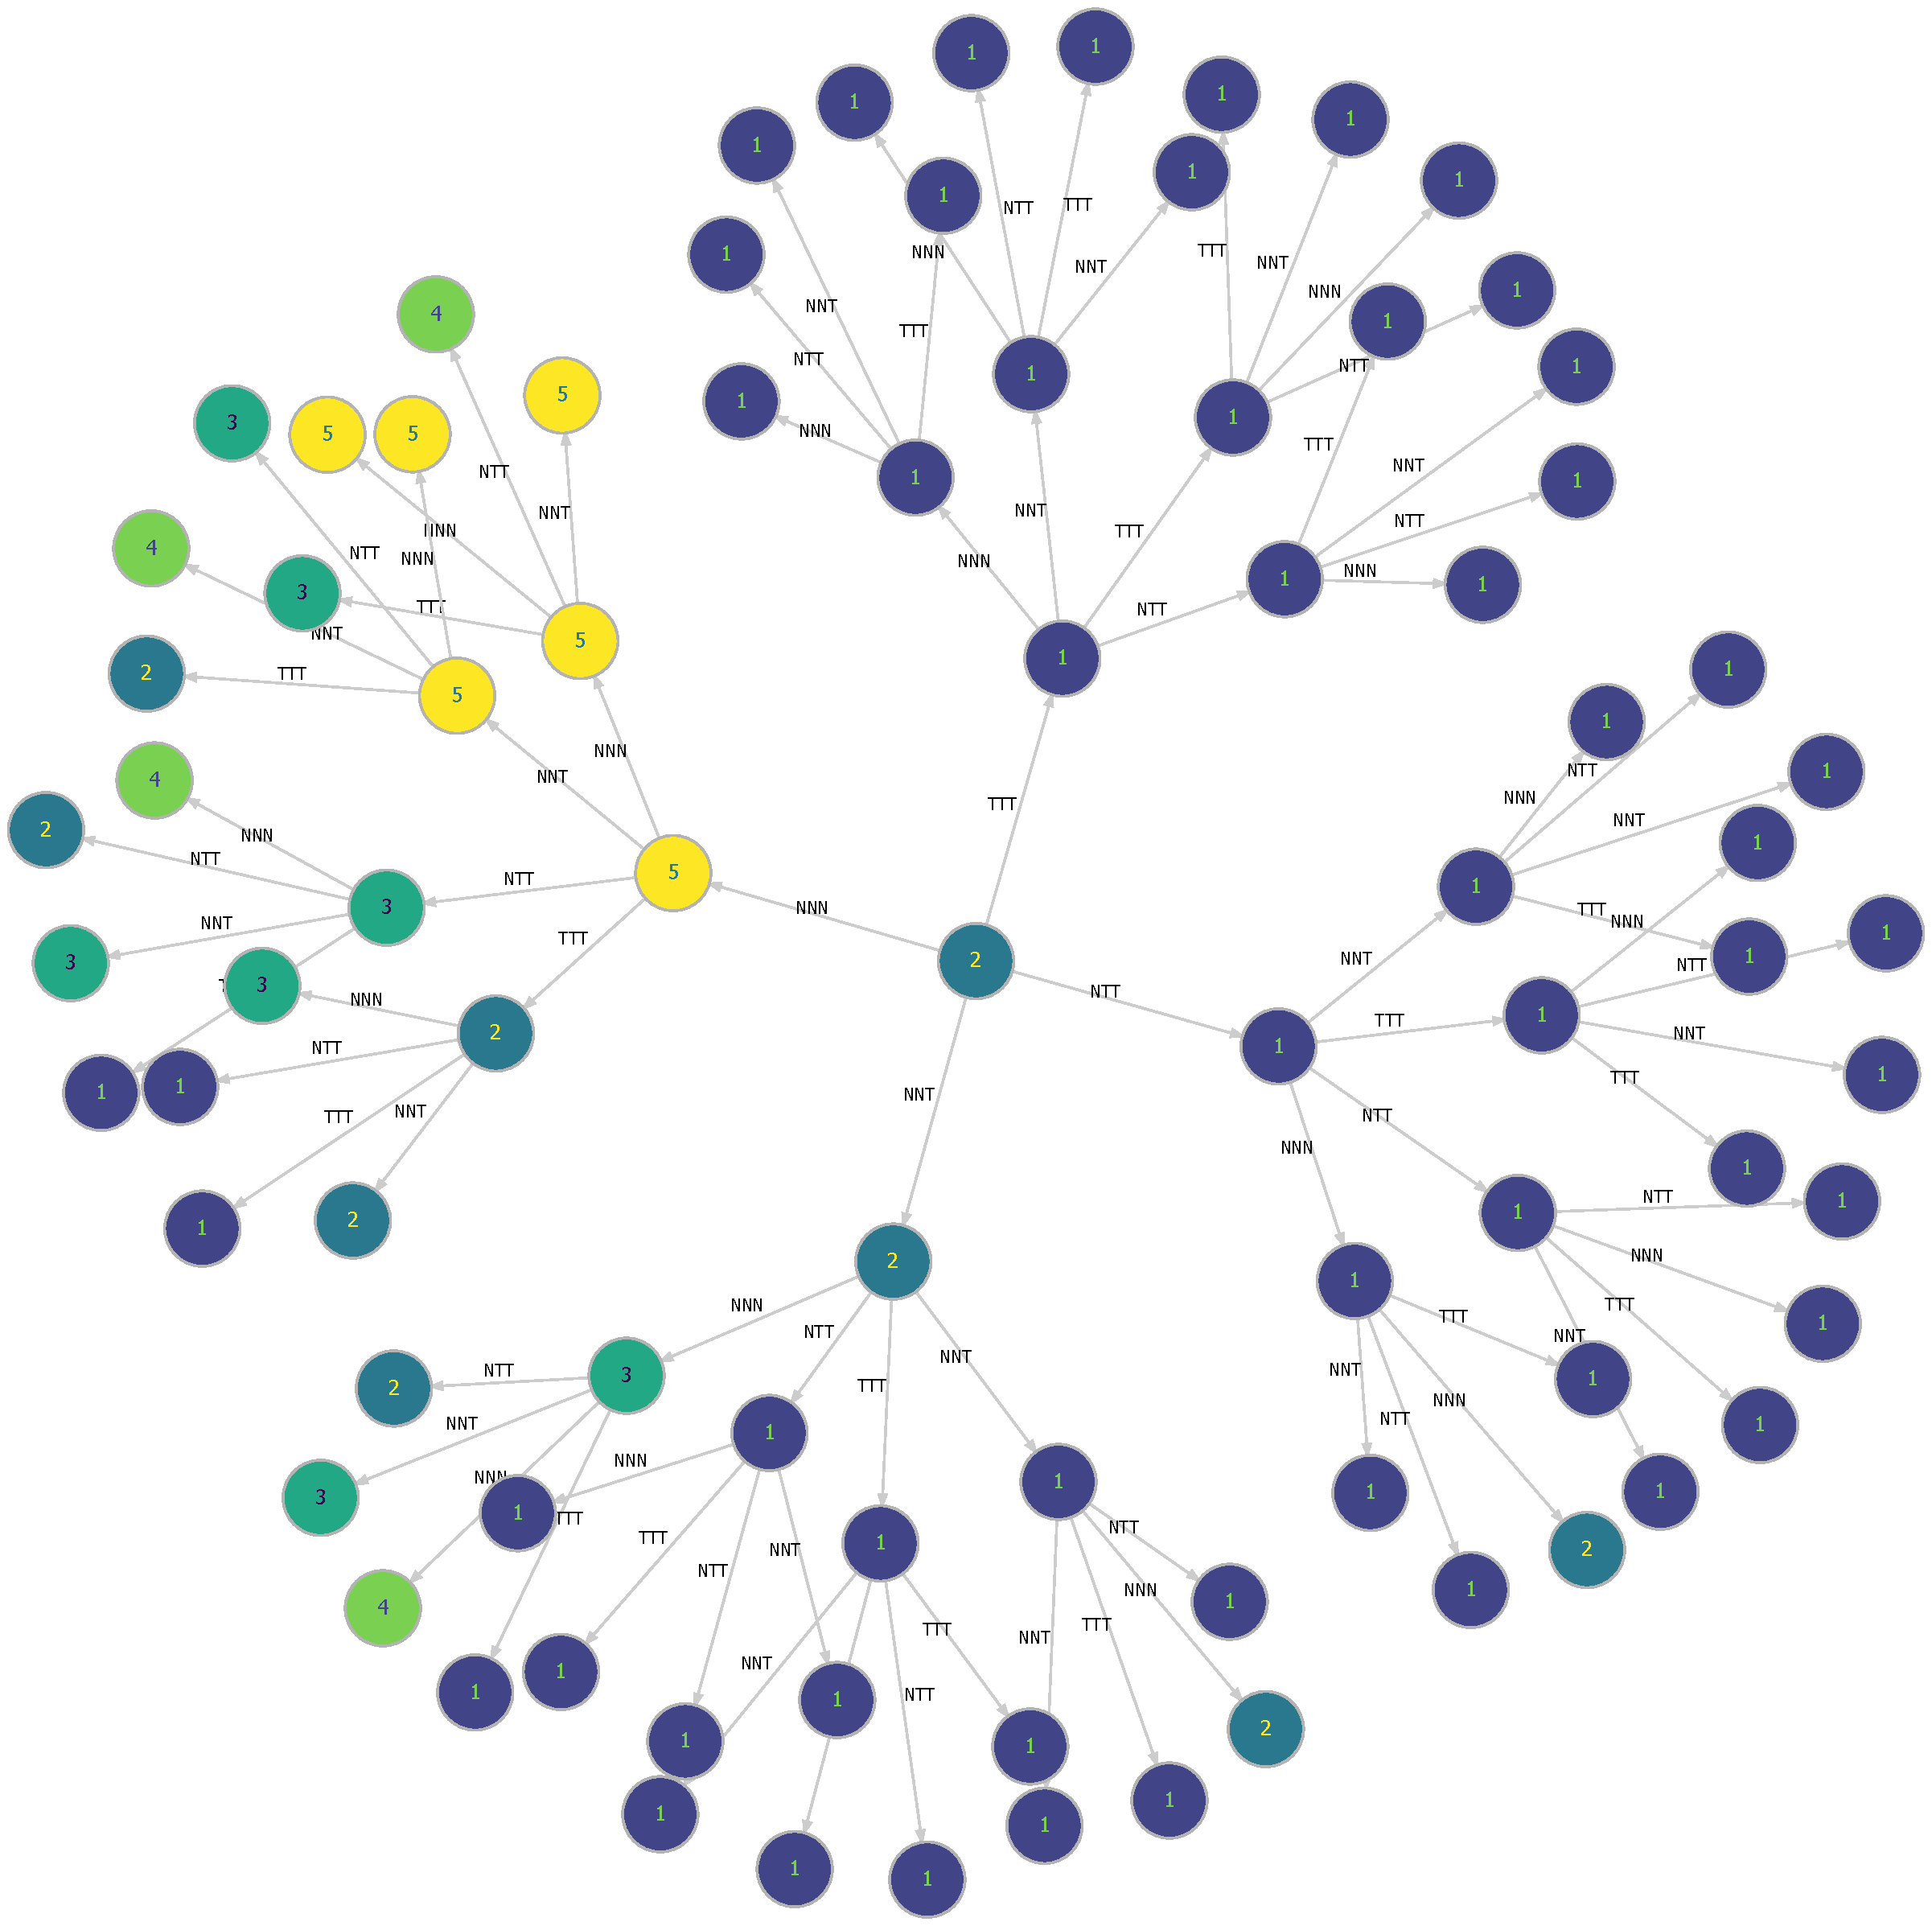
\includegraphics[width=\textwidth]{TITE-DTP-InitialExampleDTPNode}
\end{figure}

\begin{figure}[h!]
	\centering
	\caption[Initial DTP flow plot.]{Node plot of the initial DTP for the first two cohorts of our example CRM.}
	\label{fig_tite-dtp:InitialDTPExampleFlow}
	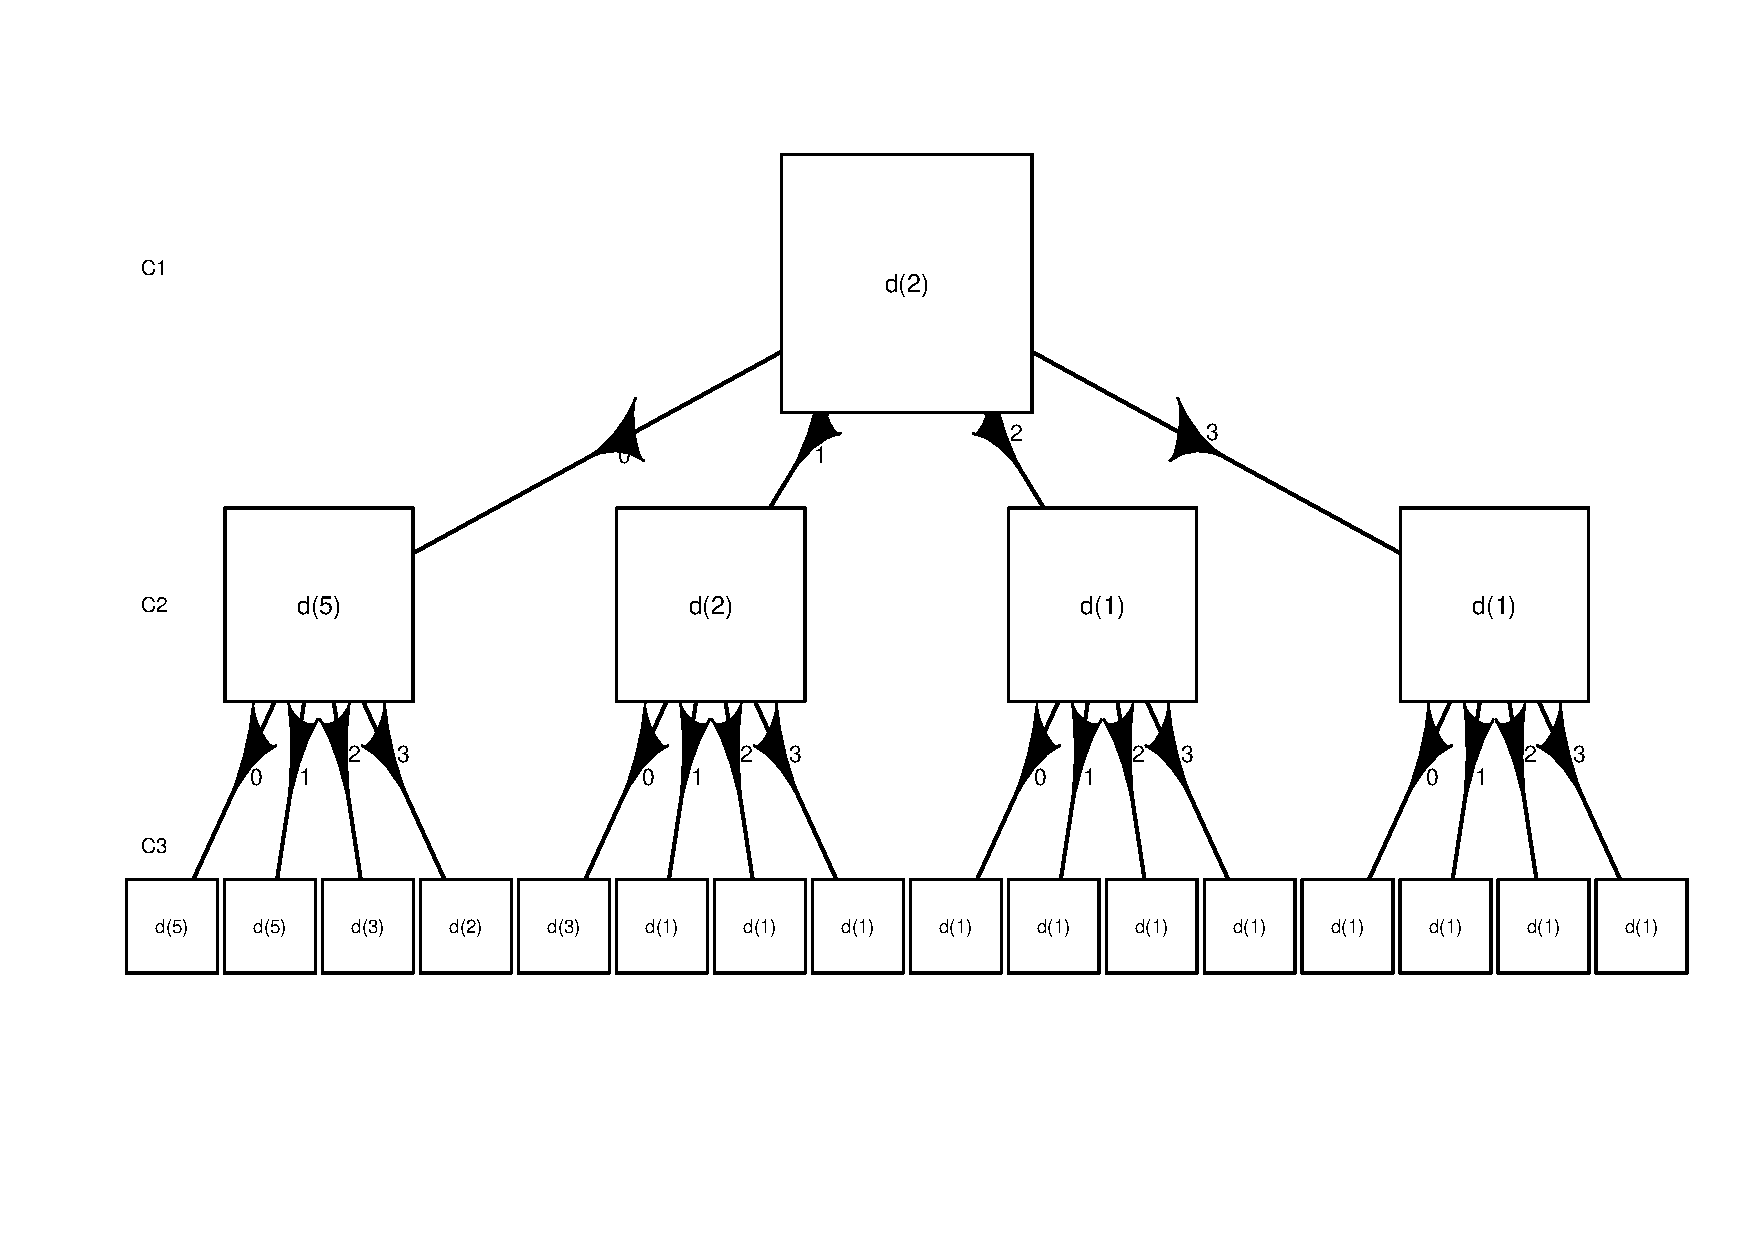
\includegraphics[width=\textwidth]{TITE-DTP-InitialExampleDTPFlow}
\end{figure}

From Table \ref{tab_tite-dtp:InitialDTPExample}, looking at pathways 33-64, we can see that if there are two or more toxicities in the first cohort the CRM will always de-escalate the dose and if there are one or more toxicities in the next two cohorts it will stay at dose-level 1. We can also see from pathways 17-32 that if we observe a toxicity event in the first cohort we will stay at the same dose-level for the next cohort. If no toxicities occur we escalate straight to the highest dose. 

Figure \ref{fig_tite-dtp:InitialDTPExampleNode} also shows the same information. The central node represents the starting dose and first cohort, from here we have 4 branches showing the various outcomes and which dose-level is allocated to the next cohort. In the case where each patient in the first cohort experience a DLT (TTT), we see that subsequent cohorts are all allocated to dose-level 1 regardless of their outcomes. Similarly, when two patients from the first cohort experience DLTs (NTT) all resulting branches show that dose-level 1 would be selected except in one case where no further DLTs occur and the CRM would escalate back to the starting dose. When one DLT occurs in the first cohort (NNT), we remain at the same dose-level. Looking at these branches if one or more DLTs are experienced in the next cohorts the dose-level is de-escalated, there is only potential for escalation in the scenario where no further DLTs occur. For the case when no DLTs occur (NNN) we see the dose for the second cohort escalated to dose-level 5. At this point, if the second cohort experiences 3 DLTs the CRM will de-escalate to dose-level 2. If there are only 2 DLTs the CRM goes to dose-level 3 and one or fewer DLTs and the next cohort will remain at dose-level 5. The flow plot, Figure \ref{fig_tite-dtp:InitialDTPExampleFlow}, only shows outcomes up to the third cohort but can be interpreted similarly to the node plot.

In combination with operating characteristics from simulations, DTPs can be used to facilitate discussions to see if the CRM can be better calibrated and is behaving optimally. In our example here there may be a few obvious things that would concern clinicians, the first being that we skip doses when escalating and the second that in the cases where lots of toxicity occurs recruitment continues. To remedy this we can include a rule not to skip untried doses and add a safety rule to stop the trial if too many toxicities occur at the lowest dose. 

In a Bayesian setting, an appropriate method to stop early would be to test the posterior distribution for the probability of toxicity. For our example here we will stop if there is at least a 90\% probability that the toxicity rate is 10\% greater than the target level at the lowest dose. This can be expressed as $P($true DLT rate at $d_1 > 0.25 + 0.1$ | observed data and prior information $) > 0.9$. 

With the addition of these two rules the DTPs can be updated, and in parallel further simulations can be produced. Table \ref{tab_tite-dtp:UpdatedDTPExample} shows the pathways for the first three cohorts. The node and flow plots were also updated, Figures \ref{fig_tite-dtp:UpdatedDTPExampleNode} and \ref{fig_tite-dtp:UpdatedDTPExampleFlow} respectively. Since we included a rule to stop in the case of excess toxicity we see several pathways terminate early so overall there are fewer pathways compared to the initial set that was produced. Here we see six different branches where it recommended that the trial stop early (pathways 32, 44, 45, 53, 54, 55 Table \ref{tab_tite-dtp:UpdatedDTPExample}). This can also be seen in Figure \ref{fig_tite-dtp:UpdatedDTPExampleNode}, we can also see three of these nodes recommend stopping before recruiting a third cohort. Using the flow plot, in Figure \ref{fig_tite-dtp:UpdatedDTPExampleFlow}, we can see that stopping is suggested when five out of the first six patients experience a DLT. Also, escalation of doses no longer skips dose-levels. With these new rules, we observe that if there are no DLTs in the first cohort the dose for the next cohort is dose-level 3 and not 5. We still observe that one toxicity in the first cohort leads to recruiting the next cohort at that same dose-level and with two or more toxicities de-escalation occurs. 

\begin{table}[h!]
	
	\caption{\label{tab_tite-dtp:UpdatedDTPExample}Updated DTPs for the first three cohorts of our example CRM with additional rules.}
	\centering
	\resizebox{\linewidth}{!}{
		\fontsize{4}{3}\selectfont
		\begin{tabular}[t]{cccccccc}
			\toprule
			\multicolumn{1}{c}{} & \multicolumn{2}{c}{Cohort 1} & \multicolumn{2}{c}{Cohort 2} & \multicolumn{2}{c}{Cohort 3} & \multicolumn{1}{c}{Cohort 4} \\
			\cmidrule(l{3pt}r{3pt}){2-3} \cmidrule(l{3pt}r{3pt}){4-5} \cmidrule(l{3pt}r{3pt}){6-7} \cmidrule(l{3pt}r{3pt}){8-8}
			Pathway & Dose & Outcomes & Dose & Outcomes & Dose & Outcomes & Dose\\
			\midrule
			\cellcolor{gray!6}{1} & \cellcolor{gray!6}{2} & \cellcolor{gray!6}{NNN} & \cellcolor{gray!6}{3} & \cellcolor{gray!6}{NNN} & \cellcolor{gray!6}{4} & \cellcolor{gray!6}{NNN} & \cellcolor{gray!6}{5}\\
			2 & 2 & NNN & 3 & NNN & 4 & NNT & 5\\
			\cellcolor{gray!6}{3} & \cellcolor{gray!6}{2} & \cellcolor{gray!6}{NNN} & \cellcolor{gray!6}{3} & \cellcolor{gray!6}{NNN} & \cellcolor{gray!6}{4} & \cellcolor{gray!6}{NTT} & \cellcolor{gray!6}{4}\\
			4 & 2 & NNN & 3 & NNN & 4 & TTT & 3\\
			\cellcolor{gray!6}{5} & \cellcolor{gray!6}{2} & \cellcolor{gray!6}{NNN} & \cellcolor{gray!6}{3} & \cellcolor{gray!6}{NNT} & \cellcolor{gray!6}{3} & \cellcolor{gray!6}{NNN} & \cellcolor{gray!6}{4}\\
			6 & 2 & NNN & 3 & NNT & 3 & NNT & 3\\
			\cellcolor{gray!6}{7} & \cellcolor{gray!6}{2} & \cellcolor{gray!6}{NNN} & \cellcolor{gray!6}{3} & \cellcolor{gray!6}{NNT} & \cellcolor{gray!6}{3} & \cellcolor{gray!6}{NTT} & \cellcolor{gray!6}{2}\\
			8 & 2 & NNN & 3 & NNT & 3 & TTT & 1\\
			\cellcolor{gray!6}{9} & \cellcolor{gray!6}{2} & \cellcolor{gray!6}{NNN} & \cellcolor{gray!6}{3} & \cellcolor{gray!6}{NTT} & \cellcolor{gray!6}{2} & \cellcolor{gray!6}{NNN} & \cellcolor{gray!6}{3}\\
			10 & 2 & NNN & 3 & NTT & 2 & NNT & 2\\
			\cellcolor{gray!6}{11} & \cellcolor{gray!6}{2} & \cellcolor{gray!6}{NNN} & \cellcolor{gray!6}{3} & \cellcolor{gray!6}{NTT} & \cellcolor{gray!6}{2} & \cellcolor{gray!6}{NTT} & \cellcolor{gray!6}{1}\\
			12 & 2 & NNN & 3 & NTT & 2 & TTT & 1\\
			\cellcolor{gray!6}{13} & \cellcolor{gray!6}{2} & \cellcolor{gray!6}{NNN} & \cellcolor{gray!6}{3} & \cellcolor{gray!6}{TTT} & \cellcolor{gray!6}{1} & \cellcolor{gray!6}{NNN} & \cellcolor{gray!6}{2}\\
			14 & 2 & NNN & 3 & TTT & 1 & NNT & 1\\
			\cellcolor{gray!6}{15} & \cellcolor{gray!6}{2} & \cellcolor{gray!6}{NNN} & \cellcolor{gray!6}{3} & \cellcolor{gray!6}{TTT} & \cellcolor{gray!6}{1} & \cellcolor{gray!6}{NTT} & \cellcolor{gray!6}{1}\\
			16 & 2 & NNN & 3 & TTT & 1 & TTT & 1\\
			\cellcolor{gray!6}{17} & \cellcolor{gray!6}{2} & \cellcolor{gray!6}{NNT} & \cellcolor{gray!6}{2} & \cellcolor{gray!6}{NNN} & \cellcolor{gray!6}{3} & \cellcolor{gray!6}{NNN} & \cellcolor{gray!6}{4}\\
			18 & 2 & NNT & 2 & NNN & 3 & NNT & 3\\
			\cellcolor{gray!6}{19} & \cellcolor{gray!6}{2} & \cellcolor{gray!6}{NNT} & \cellcolor{gray!6}{2} & \cellcolor{gray!6}{NNN} & \cellcolor{gray!6}{3} & \cellcolor{gray!6}{NTT} & \cellcolor{gray!6}{2}\\
			20 & 2 & NNT & 2 & NNN & 3 & TTT & 1\\
			\cellcolor{gray!6}{21} & \cellcolor{gray!6}{2} & \cellcolor{gray!6}{NNT} & \cellcolor{gray!6}{2} & \cellcolor{gray!6}{NNT} & \cellcolor{gray!6}{1} & \cellcolor{gray!6}{NNN} & \cellcolor{gray!6}{2}\\
			22 & 2 & NNT & 2 & NNT & 1 & NNT & 1\\
			\cellcolor{gray!6}{23} & \cellcolor{gray!6}{2} & \cellcolor{gray!6}{NNT} & \cellcolor{gray!6}{2} & \cellcolor{gray!6}{NNT} & \cellcolor{gray!6}{1} & \cellcolor{gray!6}{NTT} & \cellcolor{gray!6}{1}\\
			24 & 2 & NNT & 2 & NNT & 1 & TTT & 1\\
			\cellcolor{gray!6}{25} & \cellcolor{gray!6}{2} & \cellcolor{gray!6}{NNT} & \cellcolor{gray!6}{2} & \cellcolor{gray!6}{NTT} & \cellcolor{gray!6}{1} & \cellcolor{gray!6}{NNN} & \cellcolor{gray!6}{1}\\
			26 & 2 & NNT & 2 & NTT & 1 & NNT & 1\\
			\cellcolor{gray!6}{27} & \cellcolor{gray!6}{2} & \cellcolor{gray!6}{NNT} & \cellcolor{gray!6}{2} & \cellcolor{gray!6}{NTT} & \cellcolor{gray!6}{1} & \cellcolor{gray!6}{NTT} & \cellcolor{gray!6}{1}\\
			28 & 2 & NNT & 2 & NTT & 1 & TTT & 1\\
			\cellcolor{gray!6}{29} & \cellcolor{gray!6}{2} & \cellcolor{gray!6}{NNT} & \cellcolor{gray!6}{2} & \cellcolor{gray!6}{TTT} & \cellcolor{gray!6}{1} & \cellcolor{gray!6}{NNN} & \cellcolor{gray!6}{1}\\
			30 & 2 & NNT & 2 & TTT & 1 & NNT & 1\\
			\cellcolor{gray!6}{31} & \cellcolor{gray!6}{2} & \cellcolor{gray!6}{NNT} & \cellcolor{gray!6}{2} & \cellcolor{gray!6}{TTT} & \cellcolor{gray!6}{1} & \cellcolor{gray!6}{NTT} & \cellcolor{gray!6}{1}\\
			32 & 2 & NNT & 2 & TTT & 1 & TTT & STOP\\
			\cellcolor{gray!6}{33} & \cellcolor{gray!6}{2} & \cellcolor{gray!6}{NTT} & \cellcolor{gray!6}{1} & \cellcolor{gray!6}{NNN} & \cellcolor{gray!6}{1} & \cellcolor{gray!6}{NNN} & \cellcolor{gray!6}{2}\\
			34 & 2 & NTT & 1 & NNN & 1 & NNT & 1\\
			\cellcolor{gray!6}{35} & \cellcolor{gray!6}{2} & \cellcolor{gray!6}{NTT} & \cellcolor{gray!6}{1} & \cellcolor{gray!6}{NNN} & \cellcolor{gray!6}{1} & \cellcolor{gray!6}{NTT} & \cellcolor{gray!6}{1}\\
			36 & 2 & NTT & 1 & NNN & 1 & TTT & 1\\
			\cellcolor{gray!6}{37} & \cellcolor{gray!6}{2} & \cellcolor{gray!6}{NTT} & \cellcolor{gray!6}{1} & \cellcolor{gray!6}{NNT} & \cellcolor{gray!6}{1} & \cellcolor{gray!6}{NNN} & \cellcolor{gray!6}{1}\\
			38 & 2 & NTT & 1 & NNT & 1 & NNT & 1\\
			\cellcolor{gray!6}{39} & \cellcolor{gray!6}{2} & \cellcolor{gray!6}{NTT} & \cellcolor{gray!6}{1} & \cellcolor{gray!6}{NNT} & \cellcolor{gray!6}{1} & \cellcolor{gray!6}{NTT} & \cellcolor{gray!6}{1}\\
			40 & 2 & NTT & 1 & NNT & 1 & TTT & 1\\
			\cellcolor{gray!6}{41} & \cellcolor{gray!6}{2} & \cellcolor{gray!6}{NTT} & \cellcolor{gray!6}{1} & \cellcolor{gray!6}{NTT} & \cellcolor{gray!6}{1} & \cellcolor{gray!6}{NNN} & \cellcolor{gray!6}{1}\\
			42 & 2 & NTT & 1 & NTT & 1 & NNT & 1\\
			\cellcolor{gray!6}{43} & \cellcolor{gray!6}{2} & \cellcolor{gray!6}{NTT} & \cellcolor{gray!6}{1} & \cellcolor{gray!6}{NTT} & \cellcolor{gray!6}{1} & \cellcolor{gray!6}{NTT} & \cellcolor{gray!6}{1}\\
			44 & 2 & NTT & 1 & NTT & 1 & TTT & STOP\\
			\cellcolor{gray!6}{45} & \cellcolor{gray!6}{2} & \cellcolor{gray!6}{NTT} & \cellcolor{gray!6}{1} & \cellcolor{gray!6}{TTT} & \cellcolor{gray!6}{STOP} & \cellcolor{gray!6}{NA} & \cellcolor{gray!6}{STOP}\\
			46 & 2 & TTT & 1 & NNN & 1 & NNN & 1\\
			\cellcolor{gray!6}{47} & \cellcolor{gray!6}{2} & \cellcolor{gray!6}{TTT} & \cellcolor{gray!6}{1} & \cellcolor{gray!6}{NNN} & \cellcolor{gray!6}{1} & \cellcolor{gray!6}{NNT} & \cellcolor{gray!6}{1}\\
			48 & 2 & TTT & 1 & NNN & 1 & NTT & 1\\
			\cellcolor{gray!6}{49} & \cellcolor{gray!6}{2} & \cellcolor{gray!6}{TTT} & \cellcolor{gray!6}{1} & \cellcolor{gray!6}{NNN} & \cellcolor{gray!6}{1} & \cellcolor{gray!6}{TTT} & \cellcolor{gray!6}{1}\\
			50 & 2 & TTT & 1 & NNT & 1 & NNN & 1\\
			\cellcolor{gray!6}{51} & \cellcolor{gray!6}{2} & \cellcolor{gray!6}{TTT} & \cellcolor{gray!6}{1} & \cellcolor{gray!6}{NNT} & \cellcolor{gray!6}{1} & \cellcolor{gray!6}{NNT} & \cellcolor{gray!6}{1}\\
			52 & 2 & TTT & 1 & NNT & 1 & NTT & 1\\
			\cellcolor{gray!6}{53} & \cellcolor{gray!6}{2} & \cellcolor{gray!6}{TTT} & \cellcolor{gray!6}{1} & \cellcolor{gray!6}{NNT} & \cellcolor{gray!6}{1} & \cellcolor{gray!6}{TTT} & \cellcolor{gray!6}{STOP}\\
			54 & 2 & TTT & 1 & NTT & STOP & NA & STOP\\
			\cellcolor{gray!6}{55} & \cellcolor{gray!6}{2} & \cellcolor{gray!6}{TTT} & \cellcolor{gray!6}{1} & \cellcolor{gray!6}{TTT} & \cellcolor{gray!6}{STOP} & \cellcolor{gray!6}{NA} & \cellcolor{gray!6}{STOP}\\
			\bottomrule
	\end{tabular}}
\end{table}

\begin{figure}[h!]
	\centering
	\caption[Updated DTP node plot.]{Updated DTP node plot for the first three cohorts of our example CRM with additional rules.}
	\label{fig_tite-dtp:UpdatedDTPExampleNode}
	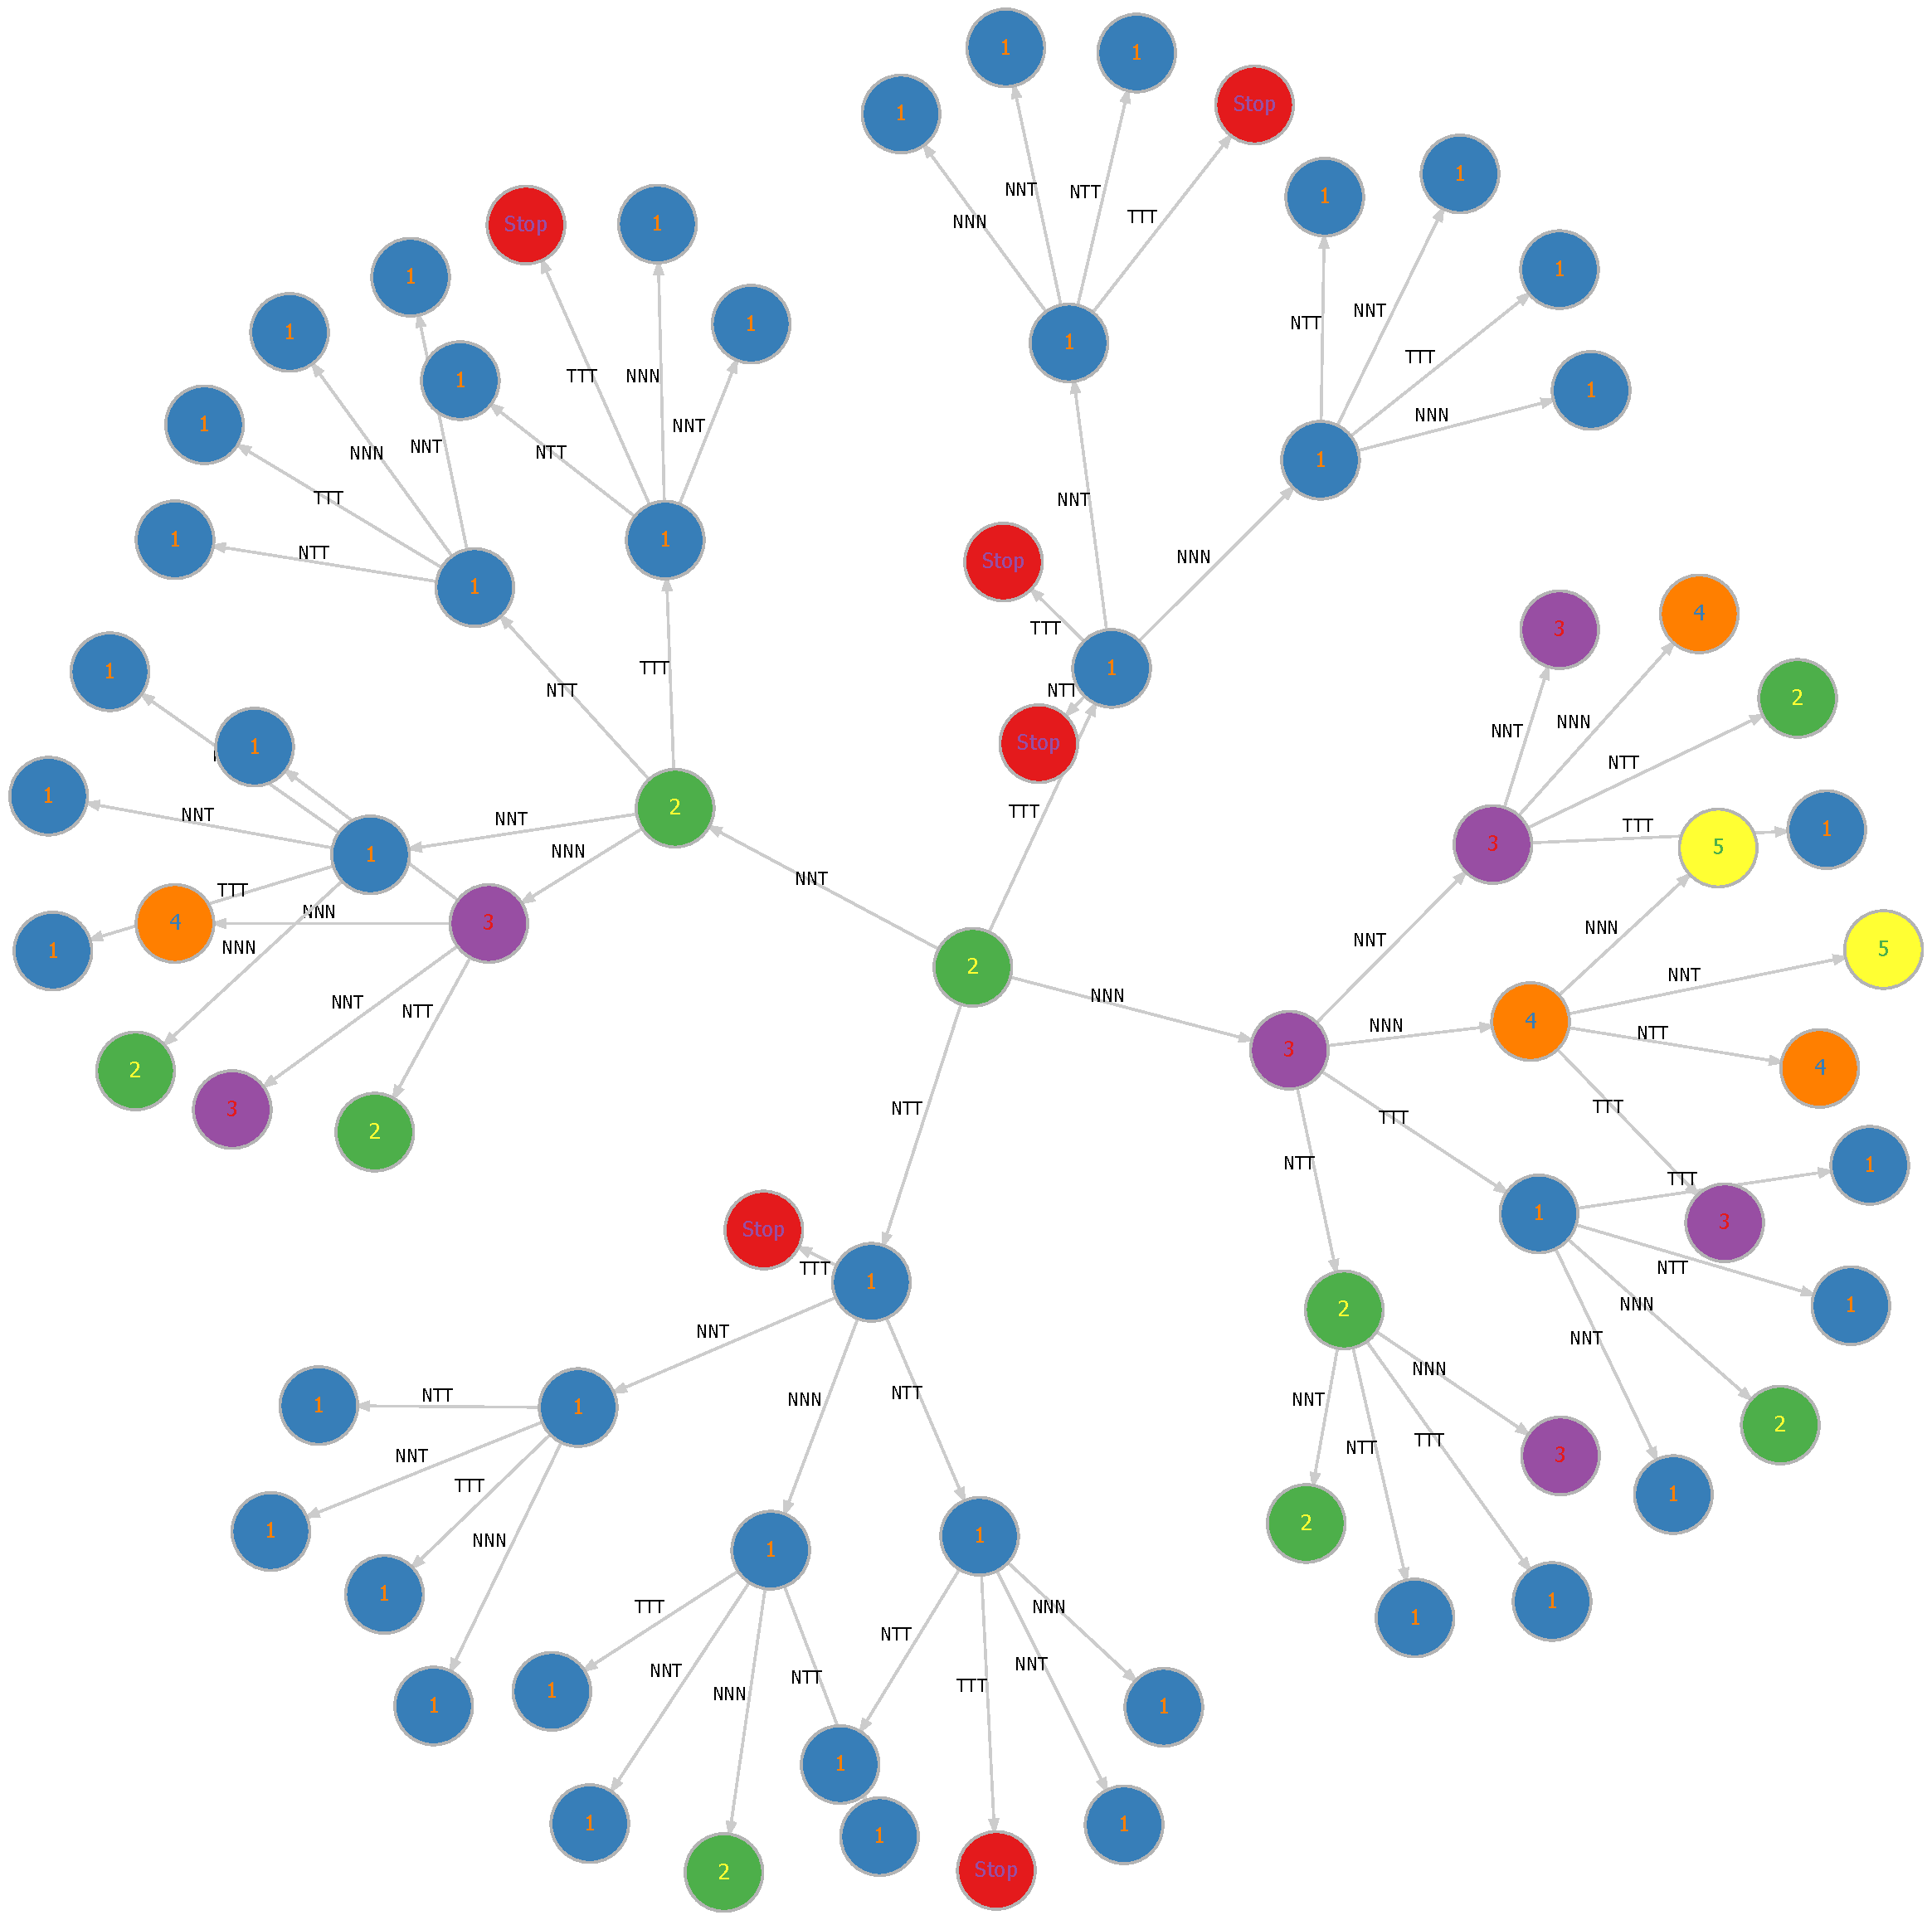
\includegraphics[width=\textwidth]{TITE-DTP-UpdatedExampleDTPNode}
\end{figure}

\begin{figure}[h!]
	\centering
	\caption[Updated DTP flow plot.]{Node plot of the updated DTP for the first two cohorts of our example CRM with additional rules.}
	\label{fig_tite-dtp:UpdatedDTPExampleFlow}
	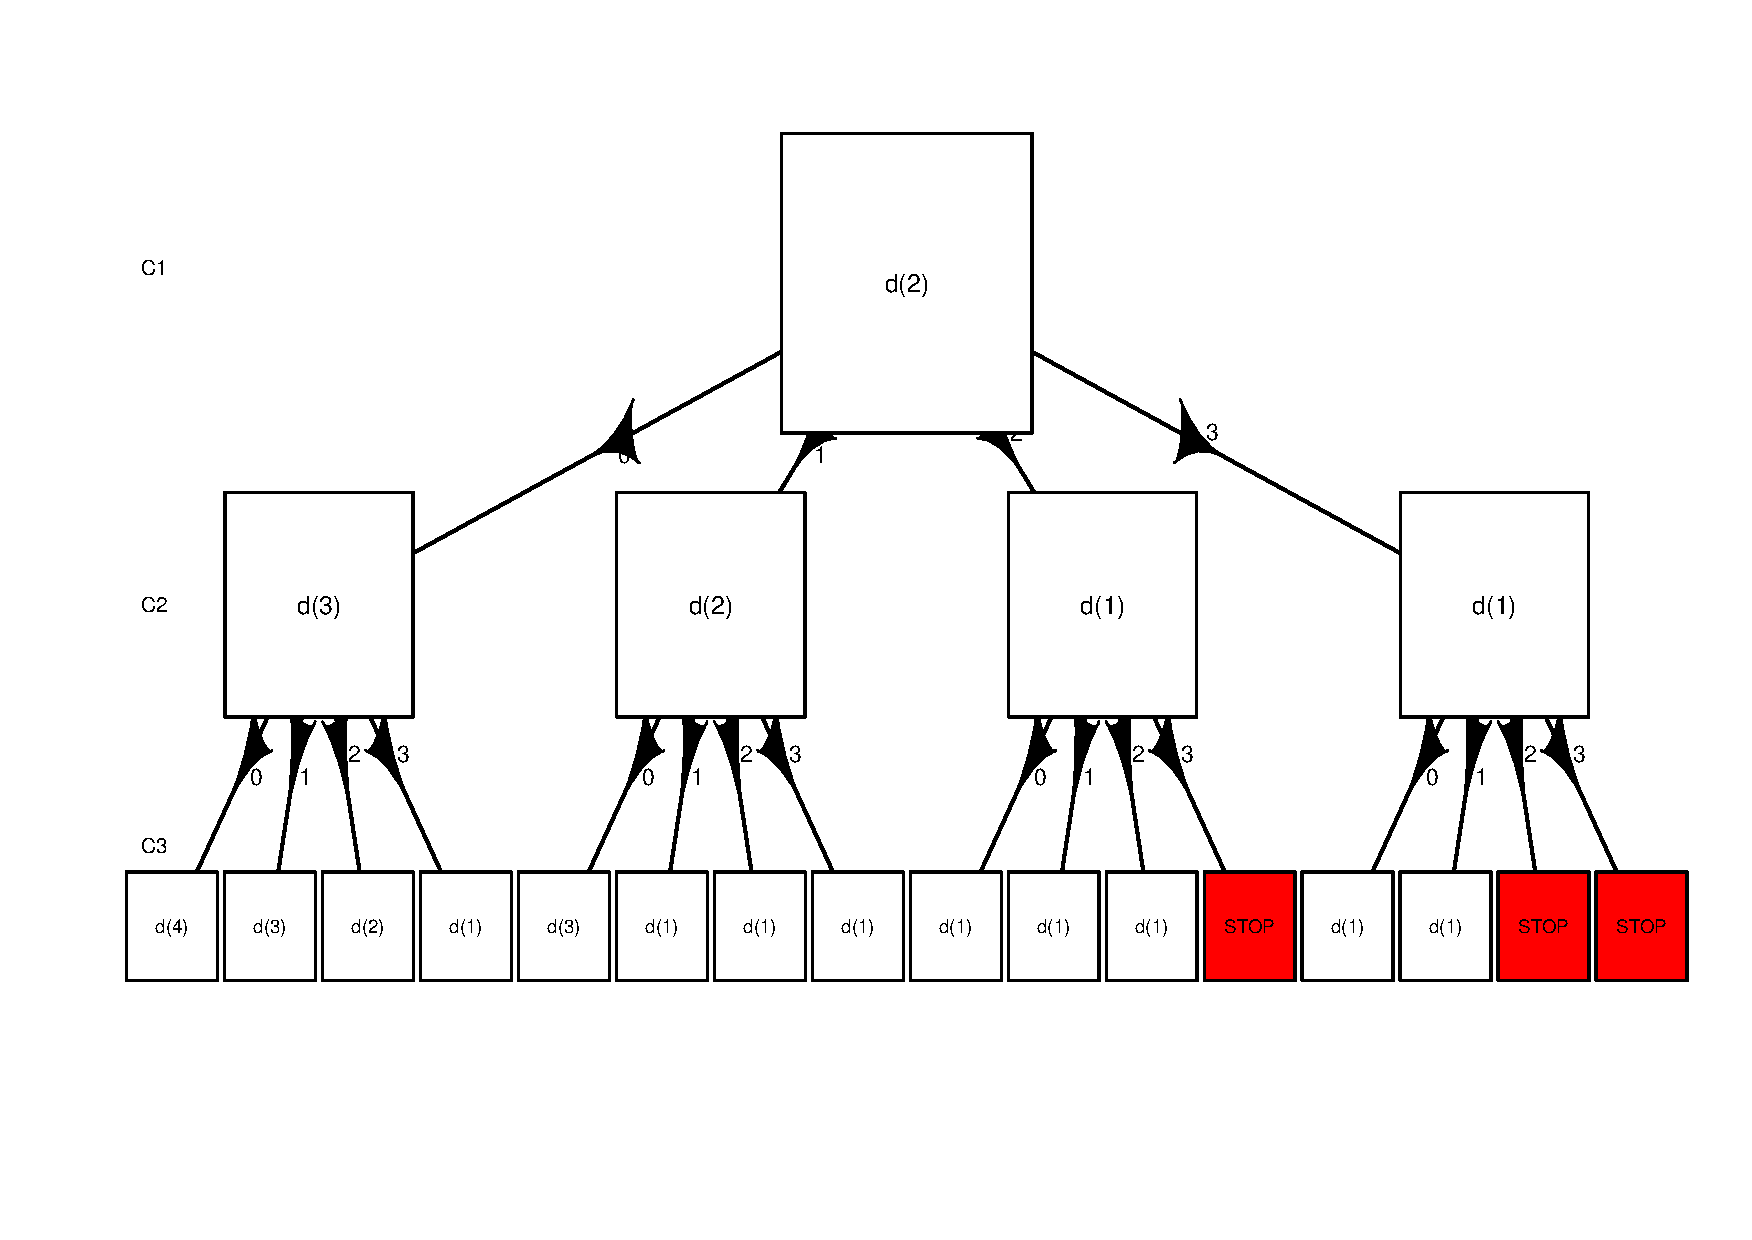
\includegraphics[width=\textwidth]{TITE-DTP-UpdatedExampleDTPFlow}
\end{figure}

At this stage, further discussions could be held about the updated DTPs and simulations. Here there may be more subtle points to discuss such as the parameters of the stopping rule. Dependent on the clinical rationale investigators may be inclined to impose either looser or stricter stopping rules. In our example, this can be done by altering the threshold values in our test of the posterior distribution of the probability of toxicity at the lowest dose. 

We also see in pathway 2 that an escalation occurs after observing a toxicity event in the previous cohort. This shows our design to be incoherent. A CRM design is considered coherent if escalation only occurs when the previous cohort experiences no DLTs and de-escalation only occurs when a DLT has been observed in the previous cohort. This property limits the risk of unnecessarily exposing patients to toxic doses whilst also ensuring patients get treated at a reasonable dose within the safety limit \cite{cheungDoseFindingContinual2011}. This became an issue due to the rule we enforced not to skip doses in escalation, the previous design without this rule was coherent. Further rules could be added to ensure the design remains coherent such that escalation will only take place if the previous cohort experience no DLTs likewise, de-escalation will only occur if the previous cohort did experience DLTs. 

Here we have highlighted how DTPs can be utilised during the initial stages of setting up a trial. Due to our example, some obvious changes could be implemented into our suggested design to improve it. However, this was just to illustrate what the pathways look like and how they can be used to facilitate discussions with the relevant clinicians and the trials team. Although we just looked at DTPs any changes being made to the design should also take into account results from the simulations. CRM designs may not be intuitively understood by clinicians but DTPs should help make them more accessible. Next, we will look at how DTPs can be used during a trial.  
%-----------------------------------
%	SUBSECTION 2
%-----------------------------------

\subsection{Using DTPs during a trial}

Dependent on the size of the dose-finding trial it will often be infeasible to present all the different pathways. In our example with only 30 patients, there were approximately 1 million different pathways. Even if we could present this data reasonably trying to decipher it may not be a worthwhile endeavour. The reason for there being so many pathways is that we have to evaluate every possible outcome for all patients at the start of the trial. As the trial progresses we observe outcomes for each patient and thus the number of pathways is reduced. This makes it possible to present DTPs for future cohorts of patients once we have accrued the outcome data of previous cohorts. 

DTPs main use in the design stage is allowing you to see how the model behaves with certain data and we can see if escalation and stopping are occurring as expected. We can then also communicate more effectively with clinicians and investigators about what our design is doing. So, once a dose-finding trial has been designed, we can continue using DTPs whilst we are accruing data to project in advance dose decisions that may occur. This has the potential to reduce the involvement of a statistician in the running and operational side of the trial. Additionally, the time between the recruitment of cohorts could also be reduced if the next recommended dose is the same dose regardless of the outcomes observed in the current cohort. It also allows the statistician to check that the model is still escalating and stopping as expected. Although at this time it may be more difficult to make changes to the design of the trial once it is underway. 

To see how this would work in practice we will use the same example as specified in Section \ref{tite-dtp:Example-DTPs} along with the stopping rule we introduced in Section \ref{tite-dtp:UsingDTPs-Calibration}. Essentially, the same design that was used to produce the DTPs in Table \ref{tab_tite-dtp:UpdatedDTPExample} and Figure \ref{fig_tite-dtp:UpdatedDTPExampleNode}. Let's assume that we run this trial and that we see outcomes for the first three cohorts that match pathway 6 in Table \ref{tab_tite-dtp:UpdatedDTPExample}. That's to say; the first cohort of patients is recruited to dose-level 2 and no toxicities are observed, cohort 2 is allocated to dose-level 3 where one toxicity is observed, then cohort 3 is allocated to dose-level 3 where again only one toxicity is observed and that leads the model recommending dose-level 3 for cohort 4. To refer to previous cohorts' outcomes we will use the nomenclature introduced by Brock \cite{brockImplementingEffToxDosefinding2017}. Outcomes for patients, either toxicity (T) or no toxicity (N) are strung behind a numeric dose-level. For instance, 2TTN denotes a cohort of three patients that were allocated to dose-level 2, two of whom experienced toxicity and one who didn't. In our example, using pathway 6 from Table \ref{tab_tite-dtp:UpdatedDTPExample}, these outcomes can be denoted as 2NNN 3NNT 3NNT. In this scenario we are unsure about the toxicity of dose-level 3 as we have seen toxicities in two separate cohorts, however, this is mainly due to only having recruited three cohorts. If we consider this our new starting point we can produce new DTPs with these previous outcomes in mind. 

Table \ref{tab_tite-dtp:UsingDuringTrialDTPs4-7} shows the new set of DTPs following previous outcomes (2NNN 3NNT 3NNT), these are also visualised in Figure \ref{fig_tite-dtp:UsingDuringTrialDTPNode4-7}. For each pathway, cohort 4 patients start at dose-level 3 as this is the model recommendation based on the previously observed outcomes. We have 64 pathways again which indicates that regardless of how many toxicities are observed the trial does not recommend stopping. See pathway 64, three patients have a toxicity event at dose-level 3 and then six have toxicities at dose-level 1. This doesn't necessarily mean that the stopping rule isn't working as intended rather due to the non-toxicities observed in the first three cohorts there would need to be more toxicity events before the rule we specified is triggered. This could be investigated further by looking at the DTPs following the outcomes of pathway 64 (i.e 2NNN 3NNT 3NNT 3TTT 1TTT 1TTT). It can also be seen if there are two or more toxicities we de-escalate and if there are no toxicities we escalate. There are also only four pathways where we end up at a higher dose in cohort 7 (pathways 1, 2, 5 and 17). Given the data we've already observed and if another toxicity occurs in cohort 4 there would need to be two cohorts of no toxicities before escalation can take place (pathway 17). 


\begin{table}[H]
	
	\caption{\label{tab_tite-dtp:UsingDuringTrialDTPs4-7}DTPs for three additional cohorts after observing outcomes for the first three cohorts.}
	\centering
	\resizebox{\linewidth}{!}{
		\fontsize{4}{3}\selectfont
		\begin{tabular}[t]{cccccccc}
			\toprule
			\multicolumn{1}{c}{} & \multicolumn{2}{c}{Cohort 4} & \multicolumn{2}{c}{Cohort 5} & \multicolumn{2}{c}{Cohort 6} & \multicolumn{1}{c}{Cohort 7} \\
			\cmidrule(l{3pt}r{3pt}){2-3} \cmidrule(l{3pt}r{3pt}){4-5} \cmidrule(l{3pt}r{3pt}){6-7} \cmidrule(l{3pt}r{3pt}){8-8}
			Pathway & Dose & Outcomes & Dose & Outcomes & Dose & Outcomes & Dose\\
			\midrule
			\cellcolor{gray!6}{1} & \cellcolor{gray!6}{3} & \cellcolor{gray!6}{NNN} & \cellcolor{gray!6}{4} & \cellcolor{gray!6}{NNN} & \cellcolor{gray!6}{4} & \cellcolor{gray!6}{NNN} & \cellcolor{gray!6}{5}\\
			2 & 3 & NNN & 4 & NNN & 4 & NNT & 4\\
			\cellcolor{gray!6}{3} & \cellcolor{gray!6}{3} & \cellcolor{gray!6}{NNN} & \cellcolor{gray!6}{4} & \cellcolor{gray!6}{NNN} & \cellcolor{gray!6}{4} & \cellcolor{gray!6}{NTT} & \cellcolor{gray!6}{3}\\
			4 & 3 & NNN & 4 & NNN & 4 & TTT & 3\\
			\cellcolor{gray!6}{5} & \cellcolor{gray!6}{3} & \cellcolor{gray!6}{NNN} & \cellcolor{gray!6}{4} & \cellcolor{gray!6}{NNT} & \cellcolor{gray!6}{4} & \cellcolor{gray!6}{NNN} & \cellcolor{gray!6}{4}\\
			6 & 3 & NNN & 4 & NNT & 4 & NNT & 3\\
			\cellcolor{gray!6}{7} & \cellcolor{gray!6}{3} & \cellcolor{gray!6}{NNN} & \cellcolor{gray!6}{4} & \cellcolor{gray!6}{NNT} & \cellcolor{gray!6}{4} & \cellcolor{gray!6}{NTT} & \cellcolor{gray!6}{3}\\
			8 & 3 & NNN & 4 & NNT & 4 & TTT & 3\\
			\cellcolor{gray!6}{9} & \cellcolor{gray!6}{3} & \cellcolor{gray!6}{NNN} & \cellcolor{gray!6}{4} & \cellcolor{gray!6}{NTT} & \cellcolor{gray!6}{3} & \cellcolor{gray!6}{NNN} & \cellcolor{gray!6}{3}\\
			10 & 3 & NNN & 4 & NTT & 3 & NNT & 3\\
			\cellcolor{gray!6}{11} & \cellcolor{gray!6}{3} & \cellcolor{gray!6}{NNN} & \cellcolor{gray!6}{4} & \cellcolor{gray!6}{NTT} & \cellcolor{gray!6}{3} & \cellcolor{gray!6}{NTT} & \cellcolor{gray!6}{2}\\
			12 & 3 & NNN & 4 & NTT & 3 & TTT & 2\\
			\cellcolor{gray!6}{13} & \cellcolor{gray!6}{3} & \cellcolor{gray!6}{NNN} & \cellcolor{gray!6}{4} & \cellcolor{gray!6}{TTT} & \cellcolor{gray!6}{2} & \cellcolor{gray!6}{NNN} & \cellcolor{gray!6}{3}\\
			14 & 3 & NNN & 4 & TTT & 2 & NNT & 2\\
			\cellcolor{gray!6}{15} & \cellcolor{gray!6}{3} & \cellcolor{gray!6}{NNN} & \cellcolor{gray!6}{4} & \cellcolor{gray!6}{TTT} & \cellcolor{gray!6}{2} & \cellcolor{gray!6}{NTT} & \cellcolor{gray!6}{2}\\
			16 & 3 & NNN & 4 & TTT & 2 & TTT & 1\\
			\cellcolor{gray!6}{17} & \cellcolor{gray!6}{3} & \cellcolor{gray!6}{NNT} & \cellcolor{gray!6}{3} & \cellcolor{gray!6}{NNN} & \cellcolor{gray!6}{3} & \cellcolor{gray!6}{NNN} & \cellcolor{gray!6}{4}\\
			18 & 3 & NNT & 3 & NNN & 3 & NNT & 3\\
			\cellcolor{gray!6}{19} & \cellcolor{gray!6}{3} & \cellcolor{gray!6}{NNT} & \cellcolor{gray!6}{3} & \cellcolor{gray!6}{NNN} & \cellcolor{gray!6}{3} & \cellcolor{gray!6}{NTT} & \cellcolor{gray!6}{3}\\
			20 & 3 & NNT & 3 & NNN & 3 & TTT & 2\\
			\cellcolor{gray!6}{21} & \cellcolor{gray!6}{3} & \cellcolor{gray!6}{NNT} & \cellcolor{gray!6}{3} & \cellcolor{gray!6}{NNT} & \cellcolor{gray!6}{3} & \cellcolor{gray!6}{NNN} & \cellcolor{gray!6}{3}\\
			22 & 3 & NNT & 3 & NNT & 3 & NNT & 3\\
			\cellcolor{gray!6}{23} & \cellcolor{gray!6}{3} & \cellcolor{gray!6}{NNT} & \cellcolor{gray!6}{3} & \cellcolor{gray!6}{NNT} & \cellcolor{gray!6}{3} & \cellcolor{gray!6}{NTT} & \cellcolor{gray!6}{2}\\
			24 & 3 & NNT & 3 & NNT & 3 & TTT & 2\\
			\cellcolor{gray!6}{25} & \cellcolor{gray!6}{3} & \cellcolor{gray!6}{NNT} & \cellcolor{gray!6}{3} & \cellcolor{gray!6}{NTT} & \cellcolor{gray!6}{2} & \cellcolor{gray!6}{NNN} & \cellcolor{gray!6}{3}\\
			26 & 3 & NNT & 3 & NTT & 2 & NNT & 2\\
			\cellcolor{gray!6}{27} & \cellcolor{gray!6}{3} & \cellcolor{gray!6}{NNT} & \cellcolor{gray!6}{3} & \cellcolor{gray!6}{NTT} & \cellcolor{gray!6}{2} & \cellcolor{gray!6}{NTT} & \cellcolor{gray!6}{1}\\
			28 & 3 & NNT & 3 & NTT & 2 & TTT & 1\\
			\cellcolor{gray!6}{29} & \cellcolor{gray!6}{3} & \cellcolor{gray!6}{NNT} & \cellcolor{gray!6}{3} & \cellcolor{gray!6}{TTT} & \cellcolor{gray!6}{2} & \cellcolor{gray!6}{NNN} & \cellcolor{gray!6}{2}\\
			30 & 3 & NNT & 3 & TTT & 2 & NNT & 1\\
			\cellcolor{gray!6}{31} & \cellcolor{gray!6}{3} & \cellcolor{gray!6}{NNT} & \cellcolor{gray!6}{3} & \cellcolor{gray!6}{TTT} & \cellcolor{gray!6}{2} & \cellcolor{gray!6}{NTT} & \cellcolor{gray!6}{1}\\
			32 & 3 & NNT & 3 & TTT & 2 & TTT & 1\\
			\cellcolor{gray!6}{33} & \cellcolor{gray!6}{3} & \cellcolor{gray!6}{NTT} & \cellcolor{gray!6}{2} & \cellcolor{gray!6}{NNN} & \cellcolor{gray!6}{3} & \cellcolor{gray!6}{NNN} & \cellcolor{gray!6}{3}\\
			34 & 3 & NTT & 2 & NNN & 3 & NNT & 3\\
			\cellcolor{gray!6}{35} & \cellcolor{gray!6}{3} & \cellcolor{gray!6}{NTT} & \cellcolor{gray!6}{2} & \cellcolor{gray!6}{NNN} & \cellcolor{gray!6}{3} & \cellcolor{gray!6}{NTT} & \cellcolor{gray!6}{2}\\
			36 & 3 & NTT & 2 & NNN & 3 & TTT & 2\\
			\cellcolor{gray!6}{37} & \cellcolor{gray!6}{3} & \cellcolor{gray!6}{NTT} & \cellcolor{gray!6}{2} & \cellcolor{gray!6}{NNT} & \cellcolor{gray!6}{2} & \cellcolor{gray!6}{NNN} & \cellcolor{gray!6}{2}\\
			38 & 3 & NTT & 2 & NNT & 2 & NNT & 2\\
			\cellcolor{gray!6}{39} & \cellcolor{gray!6}{3} & \cellcolor{gray!6}{NTT} & \cellcolor{gray!6}{2} & \cellcolor{gray!6}{NNT} & \cellcolor{gray!6}{2} & \cellcolor{gray!6}{NTT} & \cellcolor{gray!6}{1}\\
			40 & 3 & NTT & 2 & NNT & 2 & TTT & 1\\
			\cellcolor{gray!6}{41} & \cellcolor{gray!6}{3} & \cellcolor{gray!6}{NTT} & \cellcolor{gray!6}{2} & \cellcolor{gray!6}{NTT} & \cellcolor{gray!6}{1} & \cellcolor{gray!6}{NNN} & \cellcolor{gray!6}{2}\\
			42 & 3 & NTT & 2 & NTT & 1 & NNT & 1\\
			\cellcolor{gray!6}{43} & \cellcolor{gray!6}{3} & \cellcolor{gray!6}{NTT} & \cellcolor{gray!6}{2} & \cellcolor{gray!6}{NTT} & \cellcolor{gray!6}{1} & \cellcolor{gray!6}{NTT} & \cellcolor{gray!6}{1}\\
			44 & 3 & NTT & 2 & NTT & 1 & TTT & 1\\
			\cellcolor{gray!6}{45} & \cellcolor{gray!6}{3} & \cellcolor{gray!6}{NTT} & \cellcolor{gray!6}{2} & \cellcolor{gray!6}{TTT} & \cellcolor{gray!6}{1} & \cellcolor{gray!6}{NNN} & \cellcolor{gray!6}{1}\\
			46 & 3 & NTT & 2 & TTT & 1 & NNT & 1\\
			\cellcolor{gray!6}{47} & \cellcolor{gray!6}{3} & \cellcolor{gray!6}{NTT} & \cellcolor{gray!6}{2} & \cellcolor{gray!6}{TTT} & \cellcolor{gray!6}{1} & \cellcolor{gray!6}{NTT} & \cellcolor{gray!6}{1}\\
			48 & 3 & NTT & 2 & TTT & 1 & TTT & 1\\
			\cellcolor{gray!6}{49} & \cellcolor{gray!6}{3} & \cellcolor{gray!6}{TTT} & \cellcolor{gray!6}{1} & \cellcolor{gray!6}{NNN} & \cellcolor{gray!6}{2} & \cellcolor{gray!6}{NNN} & \cellcolor{gray!6}{2}\\
			50 & 3 & TTT & 1 & NNN & 2 & NNT & 2\\
			\cellcolor{gray!6}{51} & \cellcolor{gray!6}{3} & \cellcolor{gray!6}{TTT} & \cellcolor{gray!6}{1} & \cellcolor{gray!6}{NNN} & \cellcolor{gray!6}{2} & \cellcolor{gray!6}{NTT} & \cellcolor{gray!6}{1}\\
			52 & 3 & TTT & 1 & NNN & 2 & TTT & 1\\
			\cellcolor{gray!6}{53} & \cellcolor{gray!6}{3} & \cellcolor{gray!6}{TTT} & \cellcolor{gray!6}{1} & \cellcolor{gray!6}{NNT} & \cellcolor{gray!6}{1} & \cellcolor{gray!6}{NNN} & \cellcolor{gray!6}{2}\\
			54 & 3 & TTT & 1 & NNT & 1 & NNT & 1\\
			\cellcolor{gray!6}{55} & \cellcolor{gray!6}{3} & \cellcolor{gray!6}{TTT} & \cellcolor{gray!6}{1} & \cellcolor{gray!6}{NNT} & \cellcolor{gray!6}{1} & \cellcolor{gray!6}{NTT} & \cellcolor{gray!6}{1}\\
			56 & 3 & TTT & 1 & NNT & 1 & TTT & 1\\
			\cellcolor{gray!6}{57} & \cellcolor{gray!6}{3} & \cellcolor{gray!6}{TTT} & \cellcolor{gray!6}{1} & \cellcolor{gray!6}{NTT} & \cellcolor{gray!6}{1} & \cellcolor{gray!6}{NNN} & \cellcolor{gray!6}{1}\\
			58 & 3 & TTT & 1 & NTT & 1 & NNT & 1\\
			\cellcolor{gray!6}{59} & \cellcolor{gray!6}{3} & \cellcolor{gray!6}{TTT} & \cellcolor{gray!6}{1} & \cellcolor{gray!6}{NTT} & \cellcolor{gray!6}{1} & \cellcolor{gray!6}{NTT} & \cellcolor{gray!6}{1}\\
			60 & 3 & TTT & 1 & NTT & 1 & TTT & 1\\
			\cellcolor{gray!6}{61} & \cellcolor{gray!6}{3} & \cellcolor{gray!6}{TTT} & \cellcolor{gray!6}{1} & \cellcolor{gray!6}{TTT} & \cellcolor{gray!6}{1} & \cellcolor{gray!6}{NNN} & \cellcolor{gray!6}{1}\\
			62 & 3 & TTT & 1 & TTT & 1 & NNT & 1\\
			\cellcolor{gray!6}{63} & \cellcolor{gray!6}{3} & \cellcolor{gray!6}{TTT} & \cellcolor{gray!6}{1} & \cellcolor{gray!6}{TTT} & \cellcolor{gray!6}{1} & \cellcolor{gray!6}{NTT} & \cellcolor{gray!6}{1}\\
			64 & 3 & TTT & 1 & TTT & 1 & TTT & 1\\
			\bottomrule
	\end{tabular}}
\end{table}

\begin{figure}[h!]
	\centering
	\caption[DTP node plot for three additional cohorts.]{Node plot of three additional cohorts after observing outcomes for the first three cohorts.}
	\label{fig_tite-dtp:UsingDuringTrialDTPNode4-7}
	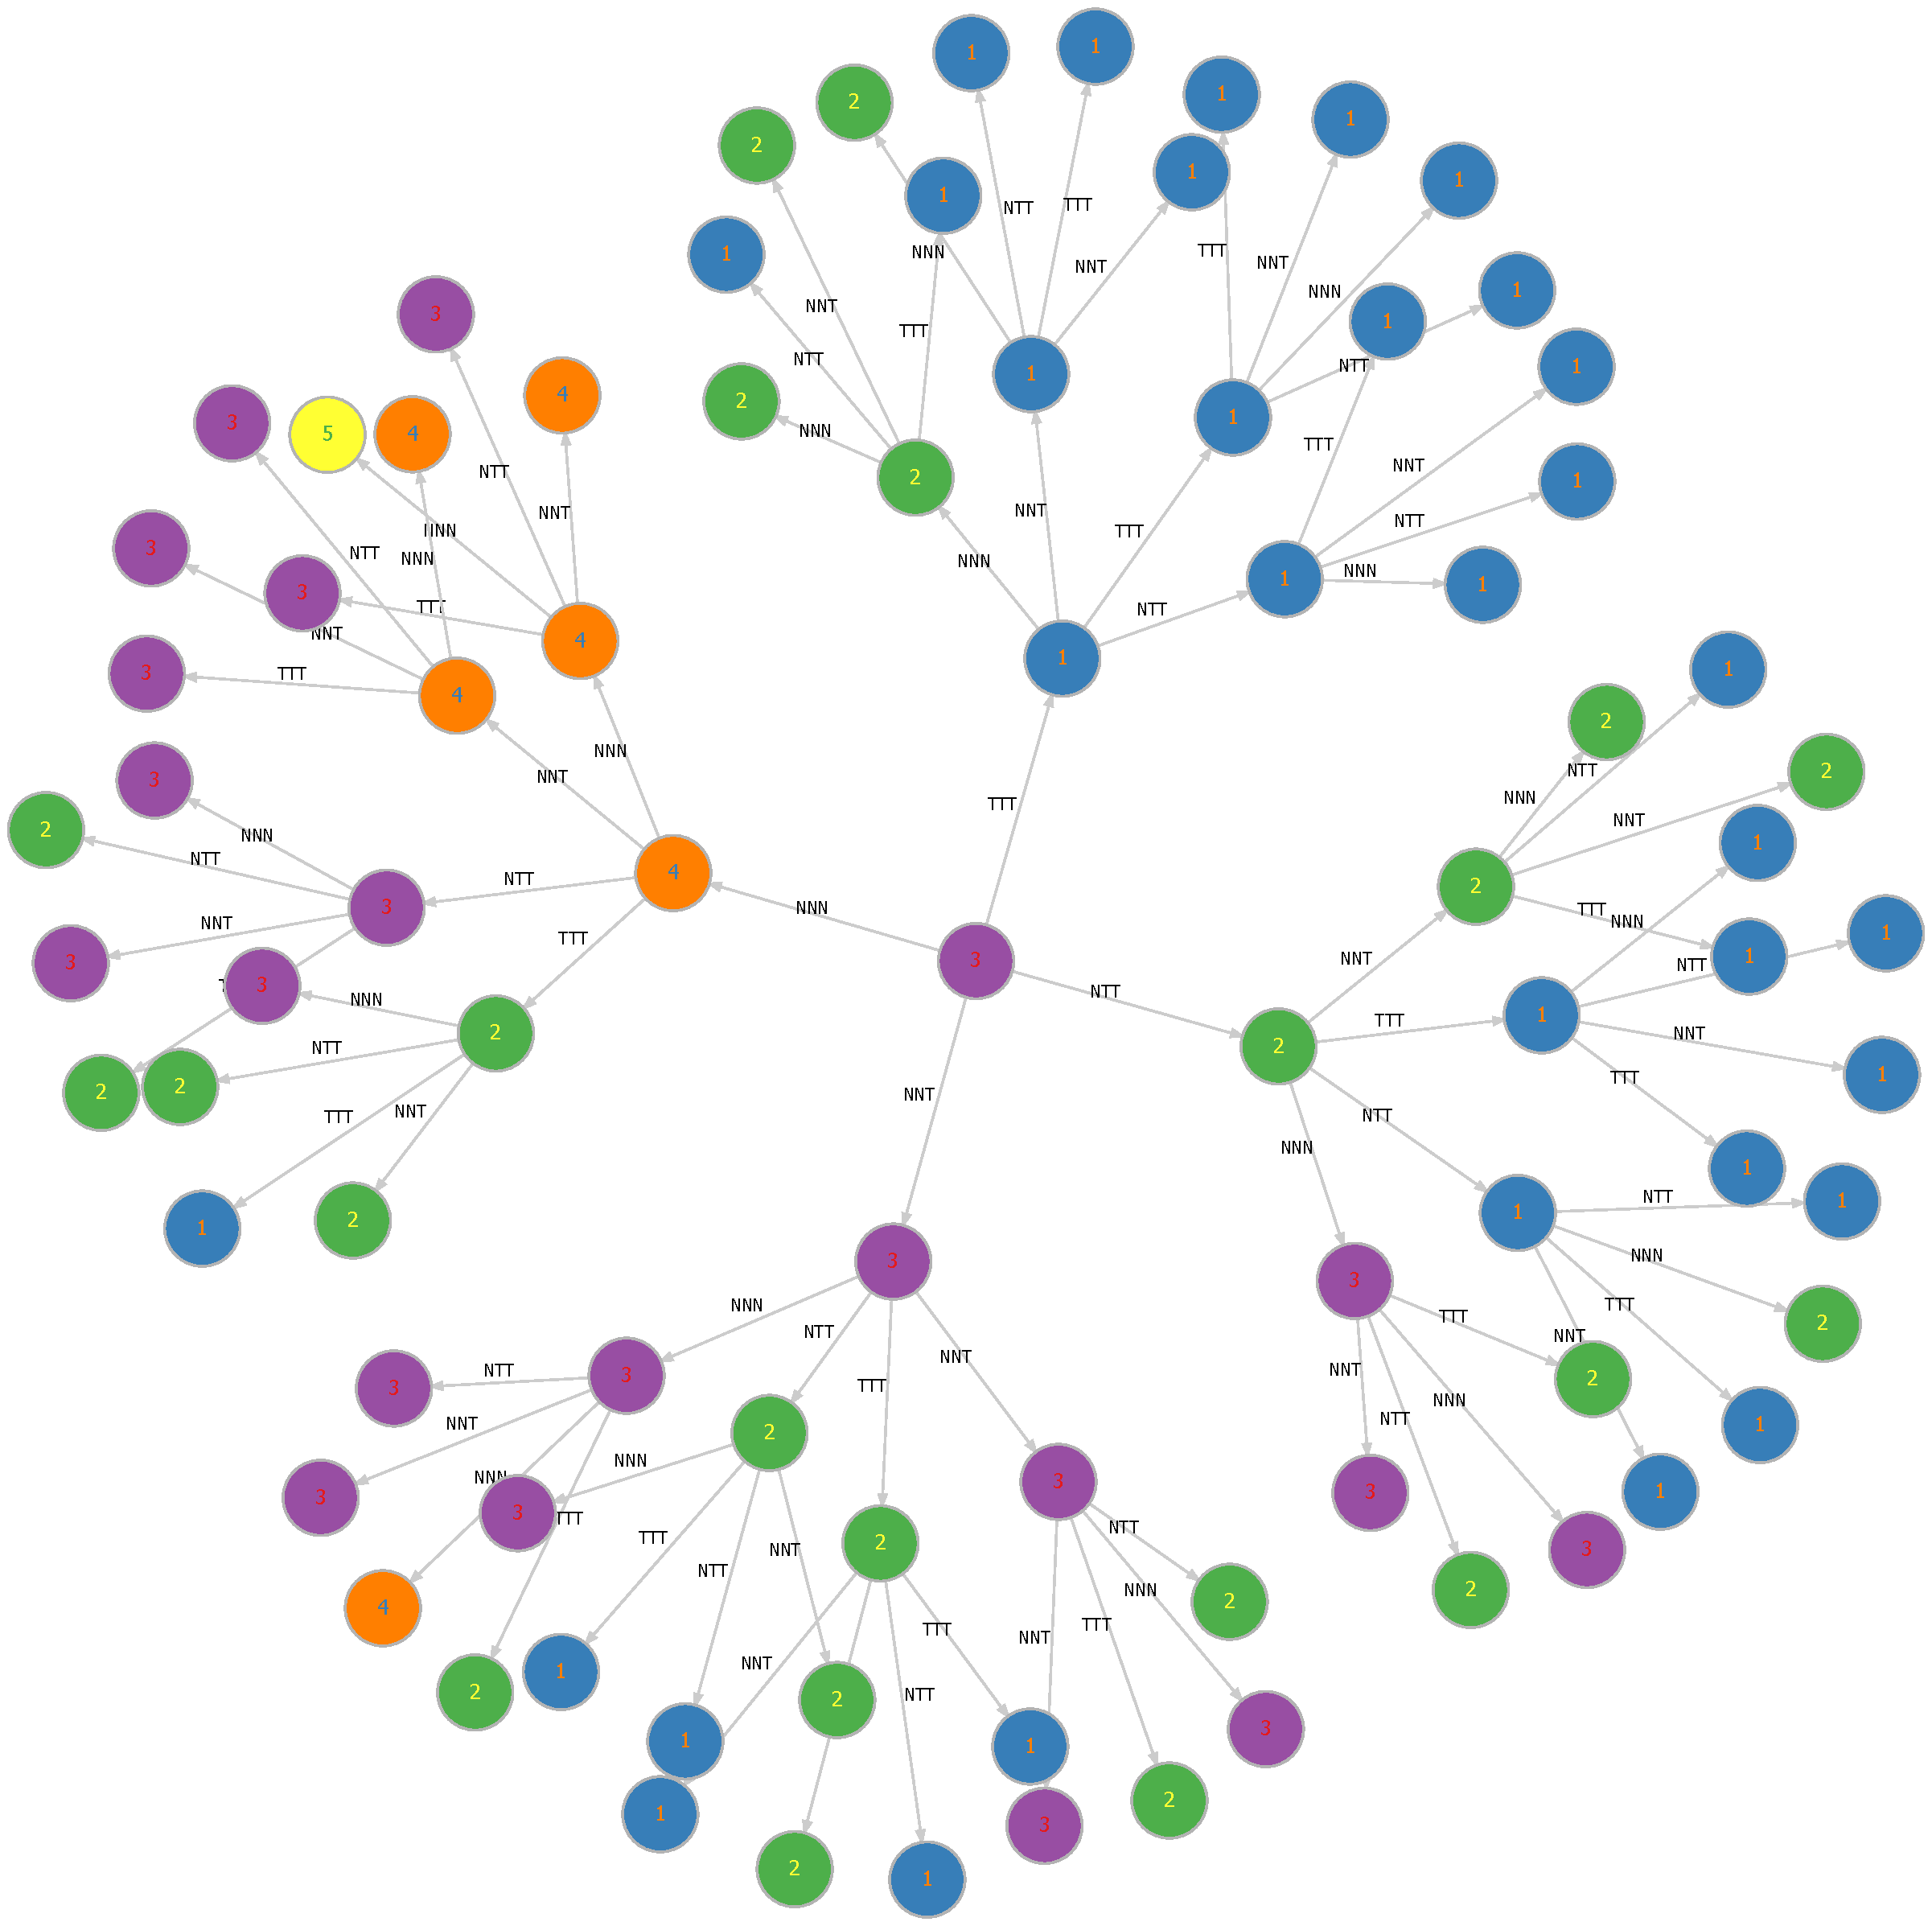
\includegraphics[width=\textwidth]{TITE-DTP-UsingDuringTrialDTPNode}
\end{figure}

Once cohort 7 is reached in the trial the DTPs can be updated again using the observed outcomes of whichever pathway occurred. These will show the potential pathways up to the 10th cohort, which is the maximum sample size in our example, and will also detail the final dose recommendation. Throughout the trial the DTPs allow us to map out what doses are recommended until the final decision. However, this has to be an iterative process as all the pathways can't be displayed simultaneously and the outcome data has to be accrued. 

DTPs can also work with non-uniform cohorts. So far our examples have been fairly simple however, in practice there may be complications with running a dose-finding trial. For instance, there may be issues with recruitment leading to long time periods between the evaluation of cohorts and dose decisions. This may be due to a number of factors such as a lack of recruiting sites, underestimation of the prevalence of disease in the patient population, or a global pandemic. One solution to this may be to reduce the cohort size and make dose decisions earlier. Model-based designs are fairly flexible at dealing with issues like these as the model could just be updated after fewer patients instead. As these considerations may not have been made in the design stages of the trial DTPs could be used as a way to evaluate any changes to cohort sizes that are made during the trial. 

We will recreate the DTPs presented earlier in this section except we will now use varying cohort sizes. These DTPs will use the same previously specified outcomes of 2NNN 3NNT 3NNT. DTPs will be calculated assuming the next three cohorts (cohorts 4,5 and 6) will only be able to recruit 2, 1 and 2 patients respectively. Table \ref{tab_tite-dtp:NonUniformDTPs4-7} lists the different pathways and they are also visualised in Figure \ref{fig_tite-dtp:NonUniformDTPNode4-7}. 

\begin{table}[H]
	
	\caption{\label{tab_tite-dtp:NonUniformDTPs4-7}DTPs for three additional cohorts with varying cohort sizes after observing outcomes for the first three cohorts.}
	\centering
	\resizebox{\linewidth}{!}{
		\fontsize{4}{3}\selectfont
		\begin{tabular}[t]{cccccccc}
			\toprule
			\multicolumn{1}{c}{} & \multicolumn{2}{c}{Cohort 4} & \multicolumn{2}{c}{Cohort 5} & \multicolumn{2}{c}{Cohort 6} & \multicolumn{1}{c}{Cohort 7} \\
			\cmidrule(l{3pt}r{3pt}){2-3} \cmidrule(l{3pt}r{3pt}){4-5} \cmidrule(l{3pt}r{3pt}){6-7} \cmidrule(l{3pt}r{3pt}){8-8}
			Pathway & Dose & Outcomes & Dose & Outcomes & Dose & Outcomes & Dose\\
			\midrule
			\cellcolor{gray!6}{1} & \cellcolor{gray!6}{3} & \cellcolor{gray!6}{NN} & \cellcolor{gray!6}{3} & \cellcolor{gray!6}{N} & \cellcolor{gray!6}{4} & \cellcolor{gray!6}{NN} & \cellcolor{gray!6}{4}\\
			2 & 3 & NN & 3 & N & 4 & NN & 4\\
			\cellcolor{gray!6}{3} & \cellcolor{gray!6}{3} & \cellcolor{gray!6}{NN} & \cellcolor{gray!6}{3} & \cellcolor{gray!6}{N} & \cellcolor{gray!6}{4} & \cellcolor{gray!6}{NT} & \cellcolor{gray!6}{3}\\
			4 & 3 & NN & 3 & N & 4 & NT & 3\\
			\cellcolor{gray!6}{5} & \cellcolor{gray!6}{3} & \cellcolor{gray!6}{NN} & \cellcolor{gray!6}{3} & \cellcolor{gray!6}{N} & \cellcolor{gray!6}{4} & \cellcolor{gray!6}{TT} & \cellcolor{gray!6}{3}\\
			6 & 3 & NN & 3 & N & 4 & TT & 3\\
			\cellcolor{gray!6}{7} & \cellcolor{gray!6}{3} & \cellcolor{gray!6}{NN} & \cellcolor{gray!6}{3} & \cellcolor{gray!6}{T} & \cellcolor{gray!6}{3} & \cellcolor{gray!6}{NN} & \cellcolor{gray!6}{3}\\
			8 & 3 & NN & 3 & T & 3 & NN & 3\\
			\cellcolor{gray!6}{9} & \cellcolor{gray!6}{3} & \cellcolor{gray!6}{NN} & \cellcolor{gray!6}{3} & \cellcolor{gray!6}{T} & \cellcolor{gray!6}{3} & \cellcolor{gray!6}{NT} & \cellcolor{gray!6}{2}\\
			10 & 3 & NN & 3 & T & 3 & NT & 2\\
			\cellcolor{gray!6}{11} & \cellcolor{gray!6}{3} & \cellcolor{gray!6}{NN} & \cellcolor{gray!6}{3} & \cellcolor{gray!6}{T} & \cellcolor{gray!6}{3} & \cellcolor{gray!6}{TT} & \cellcolor{gray!6}{2}\\
			12 & 3 & NN & 3 & T & 3 & TT & 2\\
			\cellcolor{gray!6}{13} & \cellcolor{gray!6}{3} & \cellcolor{gray!6}{NT} & \cellcolor{gray!6}{3} & \cellcolor{gray!6}{N} & \cellcolor{gray!6}{3} & \cellcolor{gray!6}{NN} & \cellcolor{gray!6}{3}\\
			14 & 3 & NT & 3 & N & 3 & NN & 3\\
			\cellcolor{gray!6}{15} & \cellcolor{gray!6}{3} & \cellcolor{gray!6}{NT} & \cellcolor{gray!6}{3} & \cellcolor{gray!6}{N} & \cellcolor{gray!6}{3} & \cellcolor{gray!6}{NT} & \cellcolor{gray!6}{2}\\
			16 & 3 & NT & 3 & N & 3 & NT & 2\\
			\cellcolor{gray!6}{17} & \cellcolor{gray!6}{3} & \cellcolor{gray!6}{NT} & \cellcolor{gray!6}{3} & \cellcolor{gray!6}{N} & \cellcolor{gray!6}{3} & \cellcolor{gray!6}{TT} & \cellcolor{gray!6}{2}\\
			18 & 3 & NT & 3 & N & 3 & TT & 2\\
			\cellcolor{gray!6}{19} & \cellcolor{gray!6}{3} & \cellcolor{gray!6}{NT} & \cellcolor{gray!6}{3} & \cellcolor{gray!6}{T} & \cellcolor{gray!6}{2} & \cellcolor{gray!6}{NN} & \cellcolor{gray!6}{2}\\
			20 & 3 & NT & 3 & T & 2 & NN & 2\\
			\cellcolor{gray!6}{21} & \cellcolor{gray!6}{3} & \cellcolor{gray!6}{NT} & \cellcolor{gray!6}{3} & \cellcolor{gray!6}{T} & \cellcolor{gray!6}{2} & \cellcolor{gray!6}{NT} & \cellcolor{gray!6}{2}\\
			22 & 3 & NT & 3 & T & 2 & NT & 2\\
			\cellcolor{gray!6}{23} & \cellcolor{gray!6}{3} & \cellcolor{gray!6}{NT} & \cellcolor{gray!6}{3} & \cellcolor{gray!6}{T} & \cellcolor{gray!6}{2} & \cellcolor{gray!6}{TT} & \cellcolor{gray!6}{1}\\
			24 & 3 & NT & 3 & T & 2 & TT & 1\\
			\cellcolor{gray!6}{25} & \cellcolor{gray!6}{3} & \cellcolor{gray!6}{TT} & \cellcolor{gray!6}{2} & \cellcolor{gray!6}{N} & \cellcolor{gray!6}{2} & \cellcolor{gray!6}{NN} & \cellcolor{gray!6}{2}\\
			26 & 3 & TT & 2 & N & 2 & NN & 2\\
			\cellcolor{gray!6}{27} & \cellcolor{gray!6}{3} & \cellcolor{gray!6}{TT} & \cellcolor{gray!6}{2} & \cellcolor{gray!6}{N} & \cellcolor{gray!6}{2} & \cellcolor{gray!6}{NT} & \cellcolor{gray!6}{2}\\
			28 & 3 & TT & 2 & N & 2 & NT & 2\\
			\cellcolor{gray!6}{29} & \cellcolor{gray!6}{3} & \cellcolor{gray!6}{TT} & \cellcolor{gray!6}{2} & \cellcolor{gray!6}{N} & \cellcolor{gray!6}{2} & \cellcolor{gray!6}{TT} & \cellcolor{gray!6}{1}\\
			30 & 3 & TT & 2 & N & 2 & TT & 1\\
			\cellcolor{gray!6}{31} & \cellcolor{gray!6}{3} & \cellcolor{gray!6}{TT} & \cellcolor{gray!6}{2} & \cellcolor{gray!6}{T} & \cellcolor{gray!6}{1} & \cellcolor{gray!6}{NN} & \cellcolor{gray!6}{2}\\
			32 & 3 & TT & 2 & T & 1 & NN & 2\\
			\cellcolor{gray!6}{33} & \cellcolor{gray!6}{3} & \cellcolor{gray!6}{TT} & \cellcolor{gray!6}{2} & \cellcolor{gray!6}{T} & \cellcolor{gray!6}{1} & \cellcolor{gray!6}{NT} & \cellcolor{gray!6}{1}\\
			34 & 3 & TT & 2 & T & 1 & NT & 1\\
			\cellcolor{gray!6}{35} & \cellcolor{gray!6}{3} & \cellcolor{gray!6}{TT} & \cellcolor{gray!6}{2} & \cellcolor{gray!6}{T} & \cellcolor{gray!6}{1} & \cellcolor{gray!6}{TT} & \cellcolor{gray!6}{1}\\
			36 & 3 & TT & 2 & T & 1 & TT & 1\\
			\bottomrule
	\end{tabular}}
\end{table}

\begin{figure}[h!]
	\centering
	\caption[DTP node plot for three additional various sized cohorts.]{Node plot of three additional cohorts with varying cohort sizes after observing outcomes for the first three cohorts.}
	\label{fig_tite-dtp:NonUniformDTPNode4-7}
	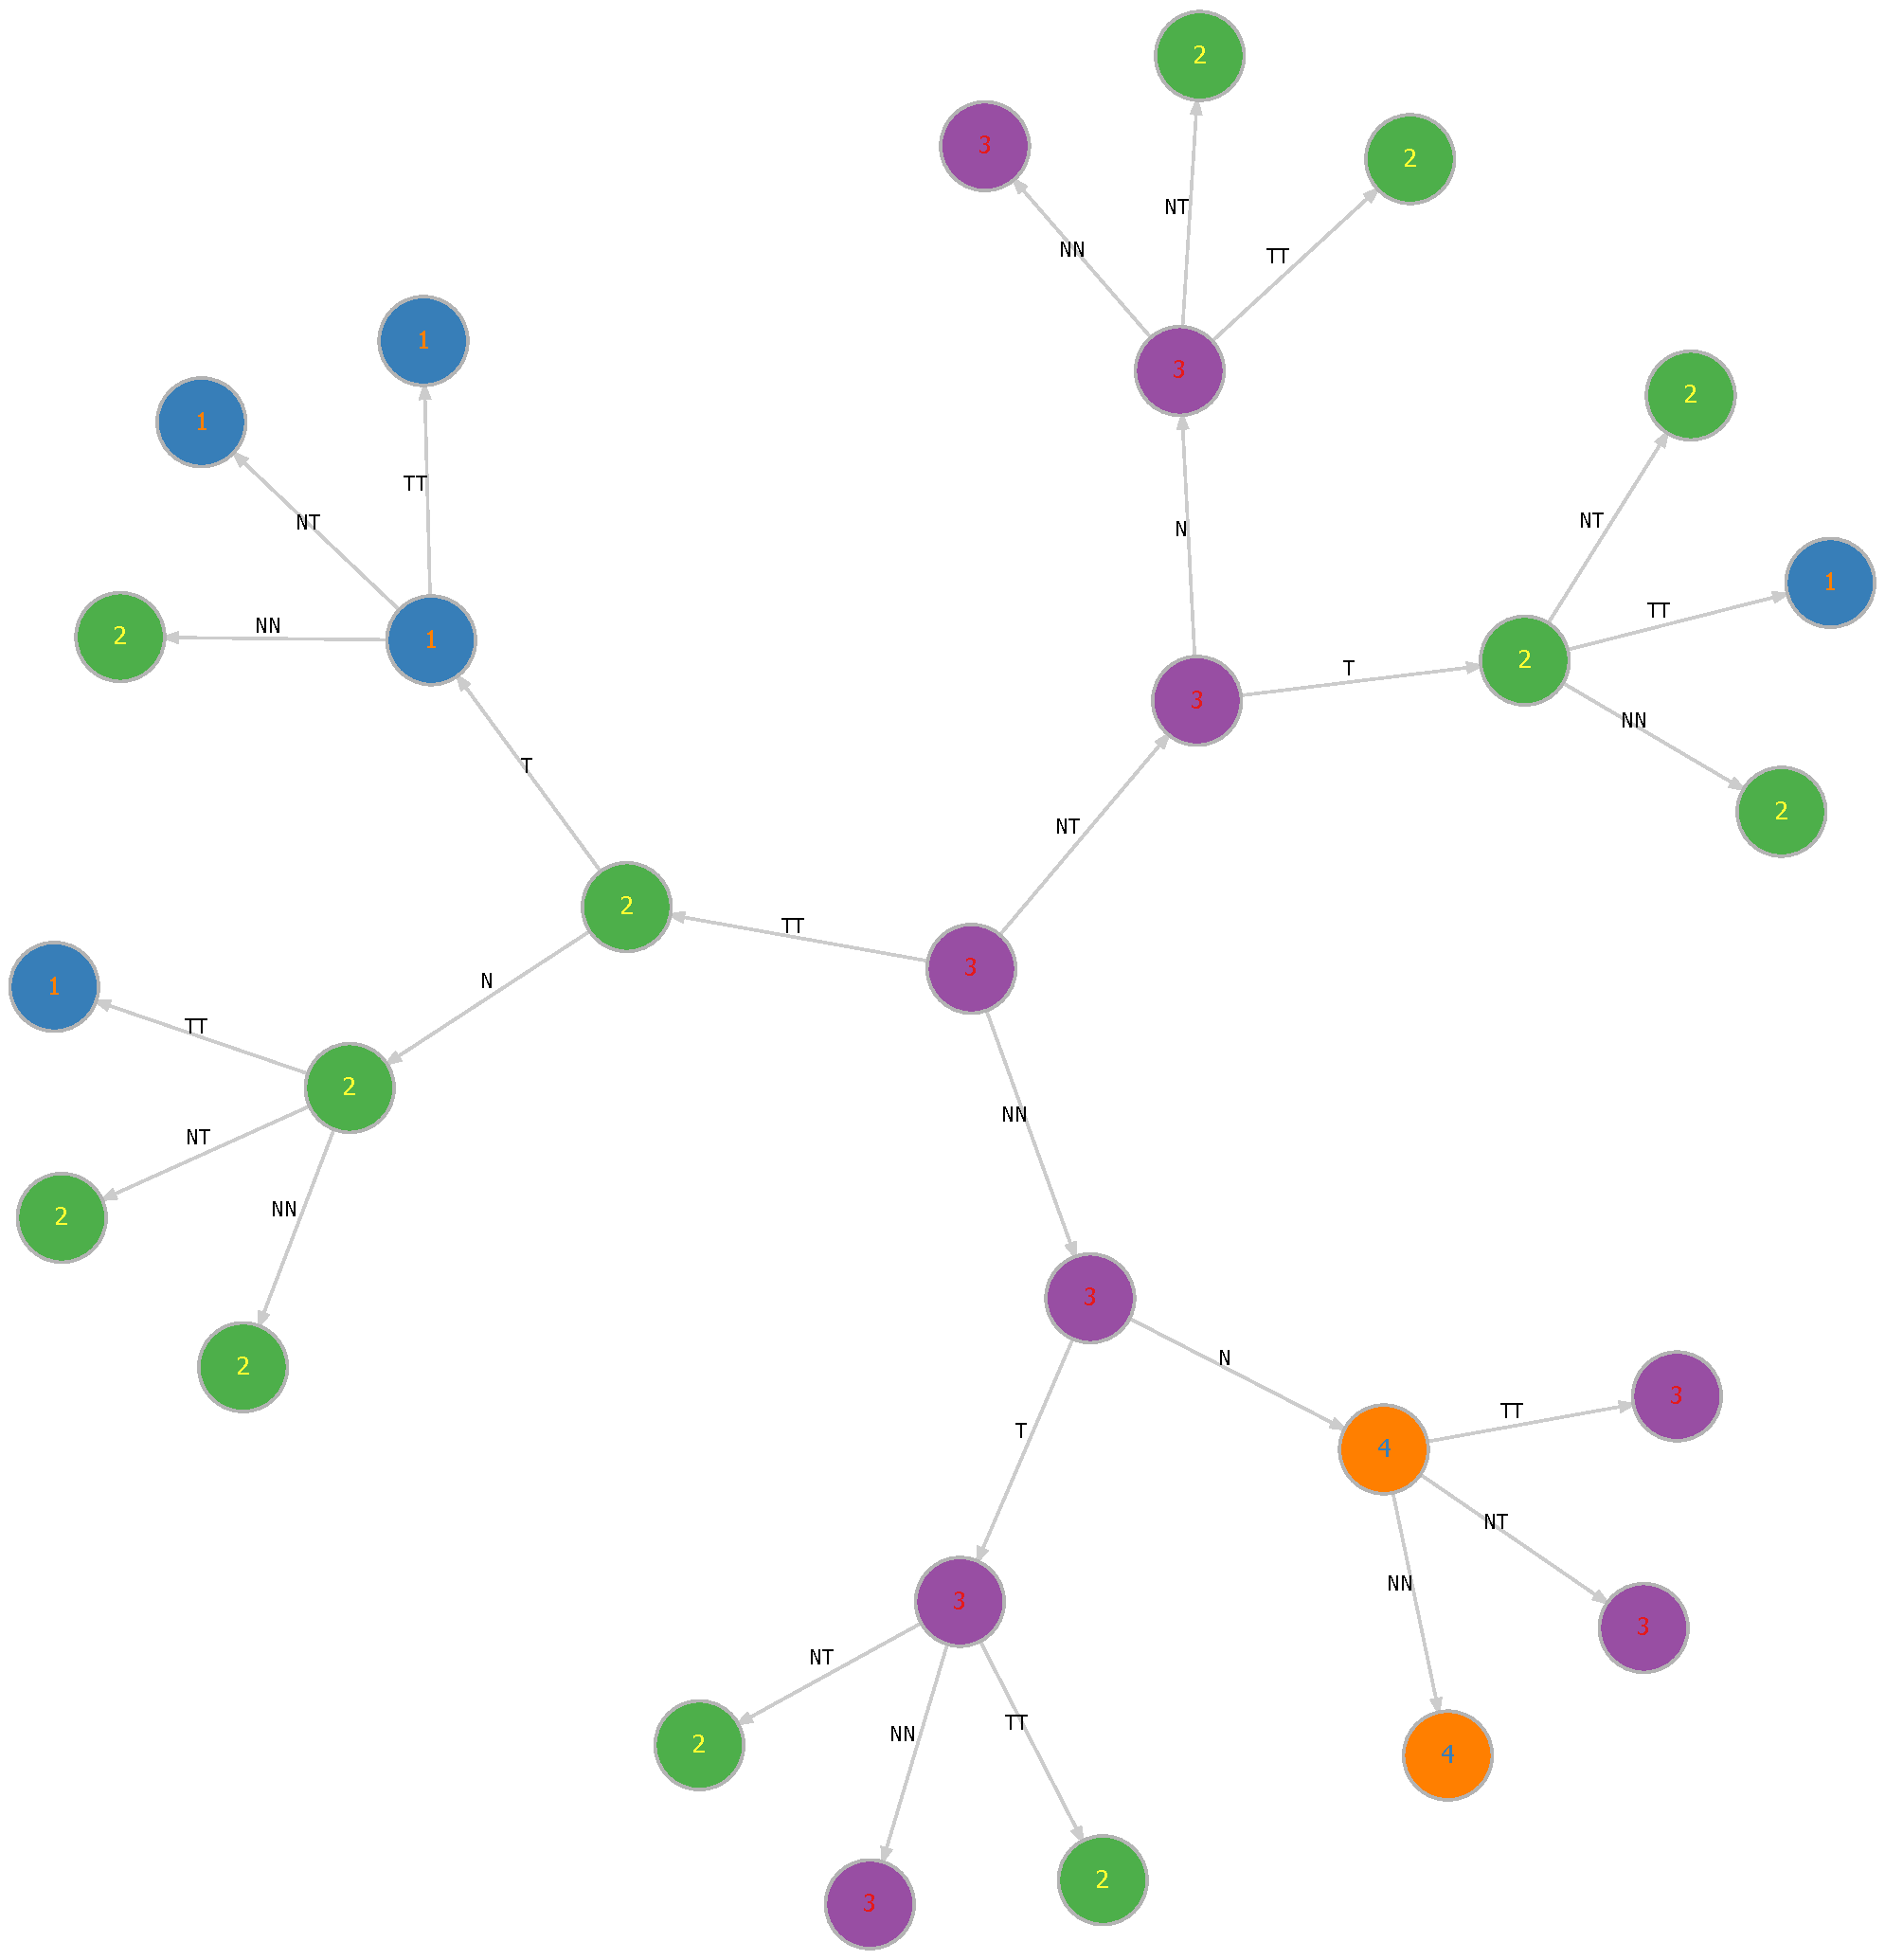
\includegraphics[width=\textwidth]{TITE-DTP-NonUniformDTPNode}
\end{figure}

These DTPs can be interpreted in the same way as before but now just correspond to a different number of patients. Where the recommended dose is set at dose-level 3 for cohort 5 we can consider these pathways equivalent to those presented earlier in Table \ref{tab_tite-dtp:UsingDuringTrialDTPs4-7} for cohort 4. As in both of these scenarios 3 patients would have been treated at dose-level 3. For instance pathways 1-6 and their recommended dose for cohort 6 in Table \ref{tab_tite-dtp:NonUniformDTPs4-7} are equivalent to pathways 1-16 and its recommended dose for cohort 5 in Table \ref{tab_tite-dtp:UsingDuringTrialDTPs4-7}, This is because in both instances 3 patients have been treated at the same dose-level and all have the same outcome. Of course, this does not always hold as a dose decision made on less data may lead to a different dose decision and hence create a different pathway. In the scenarios where two patients experience a DLT the model de-escalates and since there isn't a third patient at that dose-level 3 the following pathways will all differ from those presented previously. 

We have established how DTPs can be used during the design and calibration of a trial but also whilst it is running. They have the ability to communicate dose decisions effectively. They also help alleviate some of the potential mystery behind model based designs where clinicians and non-statisticians involved in trials may not appreciate how dose decisions are being made by a model such as the CRM. Additionally, they can also be used to assess any modifications that need to be implemented due to practical or logistical issues. It is clear DTPs are a valuable tool to incorporate in any dose-finding trial and with the escalation package by Brock \cite{brockModularApproachDose2020} they are very easy to implement, only requiring a few lines of code. 

Yap et al. \cite{yapDoseTransitionPathways2017} briefly discuss the idea of implementing DTPs in TITE-CRMs. However, limited advice or guidance was provided regarding the problems statisticians may face when trying to do this and there were no examples to refer to. In the next section, we explore the possibility of extending DTPs to work in TITE-CRMs using an illustrative example. We also discuss potential limitations and issues faced when attempting this.   

%----------------------------------------------------------------------------------------
%	SECTION 3
%----------------------------------------------------------------------------------------

\section{TITE-DTPs}
\label{tite-dtp:TITE-DTPs}

One reason why DTPs are effective is due to the simplicity of the outcomes being presented. With a CRM these outcomes are either toxicity (T) or no toxicity (N). Similarly, with a design like Wages and Tait or EffTox outcomes are either toxicity (T), efficacy (E), both toxicity and efficacy (B) or neither (N). Whilst the number of outcomes contributes to the number of potential pathways other aspects of the trial also go into determining this such as cohort size and the number of cohorts. Trying to compute and present every possible pathway is a challenge so the workaround is to just present DTPs for the initial cohorts or upcoming cohorts.  

However, when we move to the TITE setting the problem becomes more complex. TITE methodology works by using the idea of a partial tolerance event. At the time of analysis for a dose decision patients without a toxicity event who have not completed their evaluation period can be considered as having a partial tolerance. These patients can then be weighted according to how much of the evaluation period they have completed and be included in the model. If the patient completes the evaluation period without having a toxicity they have tolerated treatment and are fully weighted. This means they can be analysed and included in the model as is normally done in a standard CRM design. If a patient experiences a toxicity at any time point they are also fully weighted. 

With TITE-DTPs we still maintain the issues from normal DTPs. The number of cohorts and the cohort sizes determines the number of pathways that are produced, but now the outcome is also more complex. More specifically, just considering DTPs for a standard CRM design, patients would have either a toxicity or no toxicity now in the TITE setting we also have to account for the time each patient has spent in the trial. Patients can either have toxicity at which point they are fully weighted and just treated like they would be in a standard CRM or they could have no toxicity on day one of the evaluation period or, no toxicity on day two, no toxicity on day three etc. The number of outcomes will also depend on how long the observation window is. For example, let's assume a follow-up period of 35 days (5 weeks). Then there would be 36 different outcomes: toxicity, no toxicity (i.e. completed the evaluation period without a toxicity), no toxicity on day one, no toxicity on day two, ..., no toxicity on day 34. This problem could also be extended depending on how much precision is used in the measurement of time. 

To explore the problem further we will use an illustrative example. Consider the example trial we presented in Section \ref{tite-dtp:Example-DTPs}, except now we include a TITE component with a 35-day evaluation period. The TITE-CRM can use all the same parameters and specifications we chose for the CRM trial. When setting up a time-to-event trial we also need to specify a weight function. This function determines how patients with partial tolerances will be weighted in the TITE-CRM model. For this example, we will use a standard linear weight function where patients are weighted as a proportion of the time they have completed in the evaluation period. So, a patient who has completed 20 days would have a weight of 0.571 ($20 \div 35$). The original CRM design used cohorts of three however, due to the complexity of TITE-DTPs we will begin by looking at cohorts of one and two patients. For similar reasoning, we will also only detail pathways for the first cohort. 

%-----------------------------------
%	SUBSECTION 1
%-----------------------------------

\subsection{Cohort of one patient}
\label{tite-dtp:TITE-DTPs-c1}

First we will just look at a cohort of one patient, i.e the first patient recruited into the trial. There are 36 possible outcomes for this patient. The simplest pathway to consider is what happens when this patient has a toxicity, as the timing of the toxicity does not impact how the patient is weighted. In this scenario, the recommended dose for the next patient would be dose-level 1. So, if we see toxicity at any time point we de-escalate.   

Now in the scenario where no toxicity is observed, there are 35 different possible outcomes. Either it is day one and the patient has no toxicity, or it's day two, or day three, all the way up to no toxicity at day 35. Here we can fit the TITE-CRM model for each different outcome and see what the model will recommend as the next dose. Where the patient has between 1-19 days of follow-up the model recommends dose-level 4, anything greater than 19 and the model recommends dose-level 5.  

After calculating all possible outcomes we can produce a TITE-DTP for this cohort (Table \ref{tab_tite-dtp:TITEDTP_c1}). As previously specified the first patient starts at dose-level 2, and as there are 36 possible outcomes there are 36 pathways to the next cohort. We also extend the nomenclature of Brock et al. \cite{brockImplementingEffToxDosefinding2017} to express the different outcomes here the number in brackets represents the amount of follow-up or observation period the patient has completed. So,  N(14) indicates at 14 days the patient has had a partial tolerance event and the corresponding recommended dose for that pathway is dose-level 4.

\begin{table}[H]
	
	\caption{\label{tab_tite-dtp:TITEDTP_c1}TITE-DTP for a cohort of one.}
	\centering
	\resizebox{0.75\linewidth}{!}{
		\fontsize{4}{3}\selectfont
		\begin{tabular}[t]{cccc}
			\toprule
			\multicolumn{1}{c}{} & \multicolumn{2}{c}{Cohort 1} & \multicolumn{1}{c}{Cohort 2} \\
			\cmidrule(l{3pt}r{3pt}){2-3} \cmidrule(l{3pt}r{3pt}){4-4}
			Pathway & Dose & Outcomes & Dose\\
			\midrule
			\cellcolor{gray!6}{1} & \cellcolor{gray!6}{2} & \cellcolor{gray!6}{T} & \cellcolor{gray!6}{1}\\
			2 & 2 & N(1) & 4\\
			\cellcolor{gray!6}{3} & \cellcolor{gray!6}{2} & \cellcolor{gray!6}{N(2)} & \cellcolor{gray!6}{4}\\
			4 & 2 & N(3) & 4\\
			\cellcolor{gray!6}{5} & \cellcolor{gray!6}{2} & \cellcolor{gray!6}{N(4)} & \cellcolor{gray!6}{4}\\
			6 & 2 & N(5) & 4\\
			\cellcolor{gray!6}{7} & \cellcolor{gray!6}{2} & \cellcolor{gray!6}{N(6)} & \cellcolor{gray!6}{4}\\
			8 & 2 & N(7) & 4\\
			\cellcolor{gray!6}{9} & \cellcolor{gray!6}{2} & \cellcolor{gray!6}{N(8)} & \cellcolor{gray!6}{4}\\
			10 & 2 & N(9) & 4\\
			\cellcolor{gray!6}{11} & \cellcolor{gray!6}{2} & \cellcolor{gray!6}{N(10)} & \cellcolor{gray!6}{4}\\
			12 & 2 & N(11) & 4\\
			\cellcolor{gray!6}{13} & \cellcolor{gray!6}{2} & \cellcolor{gray!6}{N(12)} & \cellcolor{gray!6}{4}\\
			14 & 2 & N(13) & 4\\
			\cellcolor{gray!6}{15} & \cellcolor{gray!6}{2} & \cellcolor{gray!6}{N(14)} & \cellcolor{gray!6}{4}\\
			16 & 2 & N(15) & 4\\
			\cellcolor{gray!6}{17} & \cellcolor{gray!6}{2} & \cellcolor{gray!6}{N(16)} & \cellcolor{gray!6}{4}\\
			18 & 2 & N(17) & 4\\
			\cellcolor{gray!6}{19} & \cellcolor{gray!6}{2} & \cellcolor{gray!6}{N(18)} & \cellcolor{gray!6}{4}\\
			20 & 2 & N(19) & 4\\
			\cellcolor{gray!6}{21} & \cellcolor{gray!6}{2} & \cellcolor{gray!6}{N(20)} & \cellcolor{gray!6}{5}\\
			22 & 2 & N(21) & 5\\
			\cellcolor{gray!6}{23} & \cellcolor{gray!6}{2} & \cellcolor{gray!6}{N(22)} & \cellcolor{gray!6}{5}\\
			24 & 2 & N(23) & 5\\
			\cellcolor{gray!6}{25} & \cellcolor{gray!6}{2} & \cellcolor{gray!6}{N(24)} & \cellcolor{gray!6}{5}\\
			26 & 2 & N(25) & 5\\
			\cellcolor{gray!6}{27} & \cellcolor{gray!6}{2} & \cellcolor{gray!6}{N(26)} & \cellcolor{gray!6}{5}\\
			28 & 2 & N(27) & 5\\
			\cellcolor{gray!6}{29} & \cellcolor{gray!6}{2} & \cellcolor{gray!6}{N(28)} & \cellcolor{gray!6}{5}\\
			30 & 2 & N(29) & 5\\
			\cellcolor{gray!6}{31} & \cellcolor{gray!6}{2} & \cellcolor{gray!6}{N(30)} & \cellcolor{gray!6}{5}\\
			32 & 2 & N(31) & 5\\
			\cellcolor{gray!6}{33} & \cellcolor{gray!6}{2} & \cellcolor{gray!6}{N(32)} & \cellcolor{gray!6}{5}\\
			34 & 2 & N(33) & 5\\
			\cellcolor{gray!6}{35} & \cellcolor{gray!6}{2} & \cellcolor{gray!6}{N(34)} & \cellcolor{gray!6}{5}\\
			36 & 2 & N & 5\\
			\bottomrule
	\end{tabular}}
\end{table}

DTPs presented earlier in this chapter have been able to convey a lot of information. Previously with 64 pathways, we were able to specify all the possible outcomes and dose recommendations up to the 4th cohort of three patients. Whereas in the TITE setting, we have 36 just for one cohort of one patient. One way to improve on this would be to more succinctly summarise the TITE-DTP by aggregating the pathways which lead to the same recommendations. Table \ref{tab_tite-dtp:TITEDTP_c1_Sum} does this for us. 

\begin{table}[H]
	\centering
	\caption{Summary of TITE-DTP for a cohort of one.}
	\label{tab_tite-dtp:TITEDTP_c1_Sum}
	\begin{tabular}{ccccc}
		\hline
		\multicolumn{1}{l}{} &                 & \multicolumn{2}{c}{Cohort 1}   & Cohort 2 \\ 
		\cmidrule(l{3pt}r{3pt}){3-4} \cmidrule(l{3pt}r{3pt}){5-5}
		Dose                 & No. of Pathways & Outcome            & Follow-up & Dose     \\ \hline
		2                    & 1               & T                  &           & 1        \\ \hline
		\multirow{2}{*}{2}   & 19              & \multirow{2}{*}{N} & 1-19      & 4        \\
		& 16              &                    & 20-35     & 5        \\ \hline
	\end{tabular}
\end{table}

Whilst we can still apply the concept of DTPs to TITE-CRMs we can see even with just one patient and one cohort there are a lot of possible outcomes we have to look at. Also, we have used a fairly small observation period of only 5 weeks. If a larger observation period were to be used the number of pathways can get out of hand very quickly. In the next section, we explore how adding in an extra patient affects these TITE-DTPs.  

%-----------------------------------
%	SUBSECTION 2
%-----------------------------------

\subsection{Cohort of two patients}
\label{tite-dtp:TITE-DTPs-c2}
Now we consider a cohort of two patients who start at dose-level 2. As before we will consider this the first cohort of patients and only calculate pathways for the next cohort. Here the number of outcomes is a lot greater. There are three potential scenarios either both patients could have a toxicity, one of the patients could have a toxicity and one could not and finally both patients could have no toxicity. Within the two options where patients could potentially have no toxicity, there are multiple outcomes depending on how much follow-up time is observed. The different scenarios and the associated number of outcomes are: 

\begin{itemize}
	\item TT - 1 outcome 
	\item NT - 35 outcomes 
	\item NN - 630 outcomes
\end{itemize}

So, for a cohort of two patients with a follow-up period of 35 days, there are 666 possible pathways. The simplest of these is if both patients have a toxicity. Here both patients are fully weighted and when put into the model the dose recommendation is dose-level 1. 

If one patient has a toxicity and the other one doesn't there will be 35 different outcomes. One patient has a toxicity and the other has a partial tolerance event on day one, day two, day three, all the way till day 35 where they have fully tolerated the dose (i.e. N(1)T, N(2)T, N(3)T, ..., N(34)T, NT). These outcomes are just an extension of the pathways in Section \ref{tite-dtp:TITE-DTPs-c1} for one cohort of one patient, except now when we model these we include an extra patient in the model who experienced a toxicity. Table \ref{tab_tite-dtp:TITEDTP_c2NT} presents the pathways for this scenario. Here we can see regardless of how much follow-up time the patient with no toxicity has the model will always recommend de-escalating. 

\begin{table}[H]
	
	\caption{\label{tab_tite-dtp:TITEDTP_c2NT}TITE-DTP for a cohort of two for scenario NT.}
	\centering
	\resizebox{0.75\linewidth}{!}{
		\fontsize{4}{3}\selectfont
		\begin{tabular}[t]{cccc}
			\toprule
			\multicolumn{1}{c}{} & \multicolumn{2}{c}{Cohort 1} & \multicolumn{1}{c}{Cohort 2} \\
			\cmidrule(l{3pt}r{3pt}){2-3} \cmidrule(l{3pt}r{3pt}){4-4}
			Pathway & Dose & Outcomes & Dose\\
			\midrule
			\cellcolor{gray!6}{1} & \cellcolor{gray!6}{2} & \cellcolor{gray!6}{N(1)T} & \cellcolor{gray!6}{1}\\
			2 & 2 & N(2)T & 1\\
			\cellcolor{gray!6}{3} & \cellcolor{gray!6}{2} & \cellcolor{gray!6}{N(3)T} & \cellcolor{gray!6}{1}\\
			4 & 2 & N(4)T & 1\\
			\cellcolor{gray!6}{5} & \cellcolor{gray!6}{2} & \cellcolor{gray!6}{N(5)T} & \cellcolor{gray!6}{1}\\
			6 & 2 & N(6)T & 1\\
			\cellcolor{gray!6}{7} & \cellcolor{gray!6}{2} & \cellcolor{gray!6}{N(7)T} & \cellcolor{gray!6}{1}\\
			8 & 2 & N(8)T & 1\\
			\cellcolor{gray!6}{9} & \cellcolor{gray!6}{2} & \cellcolor{gray!6}{N(9)T} & \cellcolor{gray!6}{1}\\
			10 & 2 & N(10)T & 1\\
			\cellcolor{gray!6}{11} & \cellcolor{gray!6}{2} & \cellcolor{gray!6}{N(11)T} & \cellcolor{gray!6}{1}\\
			12 & 2 & N(12)T & 1\\
			\cellcolor{gray!6}{13} & \cellcolor{gray!6}{2} & \cellcolor{gray!6}{N(13)T} & \cellcolor{gray!6}{1}\\
			14 & 2 & N(14)T & 1\\
			\cellcolor{gray!6}{15} & \cellcolor{gray!6}{2} & \cellcolor{gray!6}{N(15)T} & \cellcolor{gray!6}{1}\\
			16 & 2 & N(16)T & 1\\
			\cellcolor{gray!6}{17} & \cellcolor{gray!6}{2} & \cellcolor{gray!6}{N(17)T} & \cellcolor{gray!6}{1}\\
			18 & 2 & N(18)T & 1\\
			\cellcolor{gray!6}{19} & \cellcolor{gray!6}{2} & \cellcolor{gray!6}{N(19)T} & \cellcolor{gray!6}{1}\\
			20 & 2 & N(20)T & 1\\
			\cellcolor{gray!6}{21} & \cellcolor{gray!6}{2} & \cellcolor{gray!6}{N(21)T} & \cellcolor{gray!6}{1}\\
			22 & 2 & N(22)T & 1\\
			\cellcolor{gray!6}{23} & \cellcolor{gray!6}{2} & \cellcolor{gray!6}{N(23)T} & \cellcolor{gray!6}{1}\\
			24 & 2 & N(24)T & 1\\
			\cellcolor{gray!6}{25} & \cellcolor{gray!6}{2} & \cellcolor{gray!6}{N(25)T} & \cellcolor{gray!6}{1}\\
			26 & 2 & N(26)T & 1\\
			\cellcolor{gray!6}{27} & \cellcolor{gray!6}{2} & \cellcolor{gray!6}{N(27)T} & \cellcolor{gray!6}{1}\\
			28 & 2 & N(28)T & 1\\
			\cellcolor{gray!6}{29} & \cellcolor{gray!6}{2} & \cellcolor{gray!6}{N(29)T} & \cellcolor{gray!6}{1}\\
			30 & 2 & N(30)T & 1\\
			\cellcolor{gray!6}{31} & \cellcolor{gray!6}{2} & \cellcolor{gray!6}{N(31)T} & \cellcolor{gray!6}{1}\\
			32 & 2 & N(32)T & 1\\
			\cellcolor{gray!6}{33} & \cellcolor{gray!6}{2} & \cellcolor{gray!6}{N(33)T} & \cellcolor{gray!6}{1}\\
			34 & 2 & N(34)T & 1\\
			\cellcolor{gray!6}{35} & \cellcolor{gray!6}{2} & \cellcolor{gray!6}{NT} & \cellcolor{gray!6}{1}\\
			\bottomrule
	\end{tabular}}
\end{table}

The most complicated scenario is when both patients have no toxicity. The number of outcomes for this scenario can be calculated using the combinations with replacement formula where n represents the number of follow-up days and r represents the number of patients: 

\begin{equation}
	\label{eq_tite-dtp:combinations}
	\mathbb{C}(n+r-1,r) = \frac{(n+r-1)!}{r!(n-1)!}
\end{equation}

Here we have to consider every combination of follow-up days both patients could have completed. We only consider unique combinations of days for example, N(21)N(34) would indicate one patient had been observed for 21 days and the other for 34 days, this would be the same as N(34)N(21) and so would only require one pathway. 

For our example with two patients and an observation window of 35 days, we get 630 different combinations hence the 630 pathways. Trying to show all these pathways in a table as we did before would be infeasible and hard to interpret so instead we just present the aggregate dose recommendations in Table \ref{tab_tite-dtp:TITEDTP_c2NN}. 

\begin{table}[H]
	\centering
	\caption{Summary of pathways for a cohort of two for scenario NN. }
	\label{tab_tite-dtp:TITEDTP_c2NN}
	\begin{tabular}{cccc}
		\hline
		\multicolumn{1}{l}{} & \multicolumn{1}{l}{} & \multicolumn{2}{c}{Combined no. of Follow-up Days} \\ \cline{3-4} 
		Recommend Dose & No. of Pathways & Minimum & Maximum \\ \hline
		4              & 102             & 2       & 21      \\
		5              & 528             & 20      & 70      \\ \hline
	\end{tabular}
\end{table}

We can see out of the 630 pathways, 102 recommend dose 4 for the next cohort and 528 recommend dose 5. Dose-level 4 is recommended when the combined follow-up between patients is between 2 and 21 days and dose-level 5 is recommended when the combined number of follow-up days is between 20 and 70. This presents another problem with TITE-DTPs as there is some overlap in dose recommendations depending on how much combined follow-up patients have. So, if the combined follow-up between the two patients in the cohort is 20 or 21 days they could potentially be allocated to either dose-level 4 or 5 and the way that decision is made is dependent on the split in follow-up between the two patients. This problem is also visualised in Figure \ref{fig_tite-dtp:c2NNprob}. The red lines indicate the combined follow-up time between both patients of 19 and 22 days respectively. Anything greater than 22 days combined follow-up and the model recommends dose-level 5, anything less than 19 and the recommendation is dose-level 4. In between those two time points is a bit of a grey area with the model selecting to escalate higher, to dose-level 5, with less data i.e. combined follow-up time of 20 days. Table \ref{tab_tite-dtp:TITEDTP_c2NNprob} provides a breakdown of these specific combinations. 

\begin{figure}[h!]
	\centering
	\caption[Combined follow-up and dose decisions for a cohort of two.]{Plot illustrating combined-follow up and overlap of dose recommendations for a cohort of two patients for scenario NN.}
	\label{fig_tite-dtp:c2NNprob}
	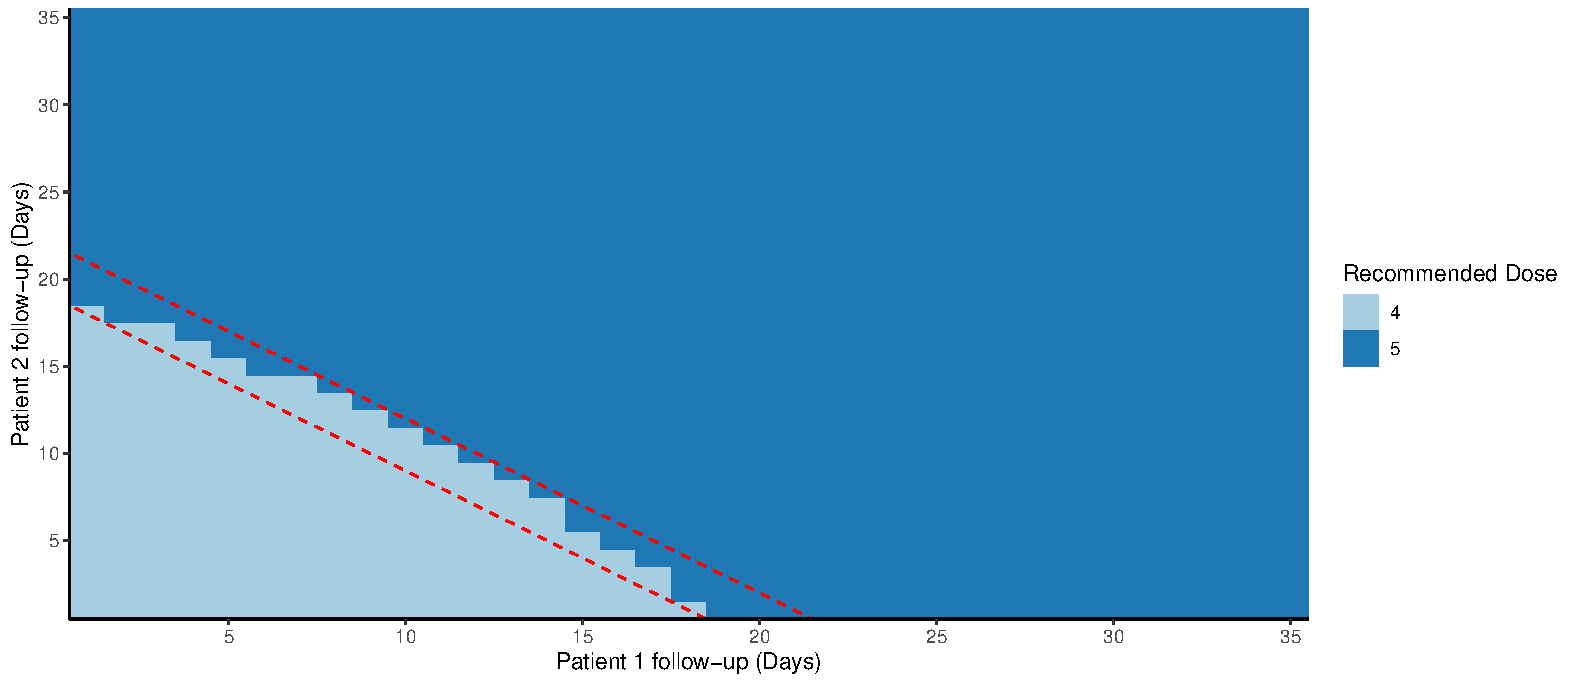
\includegraphics[width=\textwidth]{TITE-DTP-c2NN}
\end{figure}

\begin{table}[H]
	
	\caption{\label{tab_tite-dtp:TITEDTP_c2NNprob}Different dose recommendations with overlapping combined follow-up times.}
	\centering
	\fontsize{11}{13}\selectfont
	\begin{tabular}[t]{cccc}
		\toprule
		\multicolumn{2}{c}{Follow-up} & \multicolumn{2}{c}{ } \\
		\cmidrule(l{3pt}r{3pt}){1-2}
		Patient 1 & Patient 2 & Combined Follow-up & Dose Recommendation\\
		\midrule
		\cellcolor{gray!6}{1} & \cellcolor{gray!6}{19} & \cellcolor{gray!6}{20} & \cellcolor{gray!6}{5}\\
		1 & 20 & 21 & 5\\
		\cellcolor{gray!6}{2} & \cellcolor{gray!6}{18} & \cellcolor{gray!6}{20} & \cellcolor{gray!6}{5}\\
		2 & 19 & 21 & 5\\
		\cellcolor{gray!6}{3} & \cellcolor{gray!6}{17} & \cellcolor{gray!6}{20} & \cellcolor{gray!6}{4}\\
		3 & 18 & 21 & 5\\
		\cellcolor{gray!6}{4} & \cellcolor{gray!6}{16} & \cellcolor{gray!6}{20} & \cellcolor{gray!6}{4}\\
		4 & 17 & 21 & 5\\
		\cellcolor{gray!6}{5} & \cellcolor{gray!6}{15} & \cellcolor{gray!6}{20} & \cellcolor{gray!6}{4}\\
		5 & 16 & 21 & 5\\
		\cellcolor{gray!6}{6} & \cellcolor{gray!6}{14} & \cellcolor{gray!6}{20} & \cellcolor{gray!6}{4}\\
		6 & 15 & 21 & 5\\
		\cellcolor{gray!6}{7} & \cellcolor{gray!6}{13} & \cellcolor{gray!6}{20} & \cellcolor{gray!6}{4}\\
		7 & 14 & 21 & 4\\
		\cellcolor{gray!6}{8} & \cellcolor{gray!6}{12} & \cellcolor{gray!6}{20} & \cellcolor{gray!6}{4}\\
		8 & 13 & 21 & 4\\
		\cellcolor{gray!6}{9} & \cellcolor{gray!6}{11} & \cellcolor{gray!6}{20} & \cellcolor{gray!6}{4}\\
		9 & 12 & 21 & 4\\
		\cellcolor{gray!6}{10} & \cellcolor{gray!6}{10} & \cellcolor{gray!6}{20} & \cellcolor{gray!6}{4}\\
		10 & 11 & 21 & 4\\
		\bottomrule
	\end{tabular}
\end{table}

In the case where one patient has 14 days or less of follow-up, the model recommends dose-level 4, similarly, if one patient has at least 18 days of follow up the model recommends dose-level 5. Then when one patient has follow-up times of 15, 16 or 17 the model requires the second patient to have enough follow-up to make the combined total of 21 days in order to recommend dose-level 5. So, there exists some threshold whereby the model is happy to escalate further if a single patient has enough follow-up (in this case 18 days) and some critical range where the model will only escalate further if a minimum combined follow-up threshold is met (here this is between 15-17 days for one patient with the threshold being 21 days).

This could perhaps be similar to an incoherent CRM design, which escalates after observing a toxicity, except here we escalate after an inadequate amount of follow-up. It should also be noted that in practice rules may be employed to stop the trial skipping untried doses or skipping multiple doses which is what's being recommended in this case. However, that does not mean that this issue would still not occur even when selecting between two more appropriate dose-levels. 

So far we have split up the presentation of the pathways dependent on the scenario as there are too many to tabulate and present at once. Table \ref{tab_tite-dtp:TITEDTP_c2_Sum} attempts to summarise all the different pathways for a cohort of two patients. However, due to the issue earlier with the NN scenario, it is difficult to adequately summarise the combined follow-up required for the different dose decisions. Here we have opted to keep the overlap in as it allows you to see the absolute minimum and maximum combined follow-up both dose recommendations for cohort 2 require. Even though it doesn't give a specific breakdown of how many days individual patients need it may still be useful information to convey. From these values you can still determine the minimum and maximum that guarantee a specific dose as well (i.e. 18 days or less combined follow-up is dose-level 4 and 23 days or more is dose-level 5).

\begin{table}[H]
	\centering
	\caption{Summary of TITE-DTP for a cohort of two.}
	\label{tab_tite-dtp:TITEDTP_c2_Sum}
	\begin{tabular}{ccccc}
		\hline
		\multicolumn{1}{l}{} &                 & \multicolumn{2}{c}{Cohort 1}    & Cohort 2 \\ 
		\cmidrule(l{3pt}r{3pt}){3-4} \cmidrule(l{3pt}r{3pt}){5-5}
		Dose                 & No. of Pathways & Outcome             & Follow-up & Dose     \\ \hline
		2                    & 1               & TT                  &           & 1        \\ \hline
		2                    & 35              & NT                  & 1-35      & 1        \\ \hline
		\multirow{2}{*}{2}   & 102             & \multirow{2}{*}{NT} & 2-21      & 4        \\
		& 528             &                     & 19-70     & 5        \\ \hline
	\end{tabular}
\end{table}

Just by adding an extra patient to a cohort of one the number of pathways we have has increased almost 20-fold. We have also discovered when looking at specific combinations of partial tolerance events there are some inconsistencies with the way the TITE-CRM is recommending dose-levels. Finally, for completeness, we attempt producing TITE-DTPs for a cohort of 3 patients.   

%-----------------------------------
%	SUBSECTION 3
%-----------------------------------

\subsection{Cohort of three patients}
Consider instead we have a cohort of 3 patients starting at dose-level 2. Here we will explore all the possible pathways for the first cohort. With 3 patients there are four possible scenarios, the number of possible outcomes relating to each scenario is listed below: 

\begin{itemize}
	\item TTT - 1 outcome 
	\item NTT - 35 outcomes 
	\item NNT - 630 outcomes 
	\item NNN - 7770 outcomes 
\end{itemize}

In total for just the first cohort of three patients, there are 8436 pathways. The first three scenarios listed here are just extensions of what has been previously presented. When all 3 patients have a toxicity, these can just be entered into the model as fully weighted patients and the model recommends de-escalating to dose-level 1. 

The NTT scenario is the same as the cohorts of two NT scenario except now there is an extra patient in the cohort who also has a toxicity. Table \ref{tab_tite-dtp:TITEDTP_c3NTT} shows the pathways for this scenario. Regardless of the number of follow-up days the patient with no toxicity has the model will always recommend dose-level 1 if the other two patients in the cohort have toxicities. 

\begin{table}[H]
	
	\caption{\label{tab_tite-dtp:TITEDTP_c3NTT}TITE-DTP for a cohort of three for scenario NTT.}
	\centering
	\resizebox{0.75\linewidth}{!}{
		\fontsize{4}{3}\selectfont
		\begin{tabular}[t]{cccc}
			\toprule
			\multicolumn{1}{c}{} & \multicolumn{2}{c}{Cohort 1} & \multicolumn{1}{c}{Cohort 2} \\
			\cmidrule(l{3pt}r{3pt}){2-3} \cmidrule(l{3pt}r{3pt}){4-4}
			Pathway & Dose & Outcomes & Dose\\
			\midrule
			\cellcolor{gray!6}{1} & \cellcolor{gray!6}{2} & \cellcolor{gray!6}{N(1)TT} & \cellcolor{gray!6}{1}\\
			2 & 2 & N(2)TT & 1\\
			\cellcolor{gray!6}{3} & \cellcolor{gray!6}{2} & \cellcolor{gray!6}{N(3)TT} & \cellcolor{gray!6}{1}\\
			4 & 2 & N(4)TT & 1\\
			\cellcolor{gray!6}{5} & \cellcolor{gray!6}{2} & \cellcolor{gray!6}{N(5)TT} & \cellcolor{gray!6}{1}\\
			6 & 2 & N(6)TT & 1\\
			\cellcolor{gray!6}{7} & \cellcolor{gray!6}{2} & \cellcolor{gray!6}{N(7)TT} & \cellcolor{gray!6}{1}\\
			8 & 2 & N(8)TT & 1\\
			\cellcolor{gray!6}{9} & \cellcolor{gray!6}{2} & \cellcolor{gray!6}{N(9)TT} & \cellcolor{gray!6}{1}\\
			10 & 2 & N(10)TT & 1\\
			\cellcolor{gray!6}{11} & \cellcolor{gray!6}{2} & \cellcolor{gray!6}{N(11)TT} & \cellcolor{gray!6}{1}\\
			12 & 2 & N(12)TT & 1\\
			\cellcolor{gray!6}{13} & \cellcolor{gray!6}{2} & \cellcolor{gray!6}{N(13)TT} & \cellcolor{gray!6}{1}\\
			14 & 2 & N(14)TT & 1\\
			\cellcolor{gray!6}{15} & \cellcolor{gray!6}{2} & \cellcolor{gray!6}{N(15)TT} & \cellcolor{gray!6}{1}\\
			16 & 2 & N(16)TT & 1\\
			\cellcolor{gray!6}{17} & \cellcolor{gray!6}{2} & \cellcolor{gray!6}{N(17)TT} & \cellcolor{gray!6}{1}\\
			18 & 2 & N(18)TT & 1\\
			\cellcolor{gray!6}{19} & \cellcolor{gray!6}{2} & \cellcolor{gray!6}{N(19)TT} & \cellcolor{gray!6}{1}\\
			20 & 2 & N(20)TT & 1\\
			\cellcolor{gray!6}{21} & \cellcolor{gray!6}{2} & \cellcolor{gray!6}{N(21)TT} & \cellcolor{gray!6}{1}\\
			22 & 2 & N(22)TT & 1\\
			\cellcolor{gray!6}{23} & \cellcolor{gray!6}{2} & \cellcolor{gray!6}{N(23)TT} & \cellcolor{gray!6}{1}\\
			24 & 2 & N(24)TT & 1\\
			\cellcolor{gray!6}{25} & \cellcolor{gray!6}{2} & \cellcolor{gray!6}{N(25)TT} & \cellcolor{gray!6}{1}\\
			26 & 2 & N(26)TT & 1\\
			\cellcolor{gray!6}{27} & \cellcolor{gray!6}{2} & \cellcolor{gray!6}{N(27)TT} & \cellcolor{gray!6}{1}\\
			28 & 2 & N(28)TT & 1\\
			\cellcolor{gray!6}{29} & \cellcolor{gray!6}{2} & \cellcolor{gray!6}{N(29)TT} & \cellcolor{gray!6}{1}\\
			30 & 2 & N(30)TT & 1\\
			\cellcolor{gray!6}{31} & \cellcolor{gray!6}{2} & \cellcolor{gray!6}{N(31)TT} & \cellcolor{gray!6}{1}\\
			32 & 2 & N(32)TT & 1\\
			\cellcolor{gray!6}{33} & \cellcolor{gray!6}{2} & \cellcolor{gray!6}{N(33)TT} & \cellcolor{gray!6}{1}\\
			34 & 2 & N(34)TT & 1\\
			\cellcolor{gray!6}{35} & \cellcolor{gray!6}{2} & \cellcolor{gray!6}{NTT} & \cellcolor{gray!6}{1}\\
			\bottomrule
	\end{tabular}}
\end{table}

Similarly, the NNT scenario is an extension of the NN scenario for a cohort of two patients. We add an extra patient who experiences a toxicity and fit the same models and observe the outcomes. Table \ref{tab_tite-dtp:TITEDTP_c3NNT} shows a summary of the 630 possible pathways. We can see that the majority of the time the model recommends de-escalating. However, there are six pathways where the model recommends staying at the same dose, dose-level 2. this is when the combined follow-up time from the two patients who don't have a toxicity is between 67 and 70 days. We also no longer have that inconsistency issue that we saw before where different dose decisions were being made on the same amount of follow-up time dependent on the split of days between patients. Here the TITE DTP is more clear and a combined follow-up time of 66 days or less leads to de-escalation otherwise the next dose should be recruited at the same dose-level.

\begin{table}[H]
	\centering
	\caption{Summary of pathways for a cohort of three for scenario NNT. }
	\label{tab_tite-dtp:TITEDTP_c3NNT}
	\begin{tabular}{cccc}
		\hline
		\multicolumn{1}{l}{} & \multicolumn{1}{l}{} & \multicolumn{2}{c}{Combined no. of Follow-up Days} \\ \cline{3-4} 
		Recommend Dose & No. of Pathways & Minimum & Maximum \\ \hline
		1              & 624             & 2       & 66      \\
		2              & 6               & 67      & 70      \\ \hline
	\end{tabular}
\end{table}

When an additional patient is added to the cohort, the most complicated scenario is when all patients in the cohort experience no toxicity. With 3 patients and 35 days follow-up, 7770 different possible combinations of follow-up days can be observed. The results from fitting all these models are presented in Table \ref{tab_tite-dtp:TITEDTP_c3NNN}. In this scenario, if the combined number of follow-up between the three patients is between 3 and 23 days the model will recommend dose-level 4 and if it's above 27 dose-level 5 will be recommended. Again we see the same problem as before with a cohort of two patients for the NN scenario. There appears to be some overlap in dose decisions for certain combinations of follow-up days between the three patients. Anything between 24 and 26 days may result in either a recommendation of dose-level 4 or 5 depending on the split of follow-up time between the three patients. Figure \ref{fig_tite-dtp:c3NNNprob} also provides a 3D illustration of these pathways with each dot representing a different decision, and the colour corresponding to the dose recommended. A dark blue dot indicates dose-level 4 and light blue is dose-level 5.  

\begin{table}[H]
	\centering
	\caption{Summary of pathways for a cohort of three for scenario NNN. }
	\label{tab_tite-dtp:TITEDTP_c3NNN}
	\begin{tabular}{cccc}
		\hline
		\multicolumn{1}{l}{} & \multicolumn{1}{l}{} & \multicolumn{2}{c}{Combined no. of Follow-up Days} \\ \cline{3-4} 
		Recommend Dose & No. of Pathways & Minimum & Maximum \\ \hline
		4              & 484             & 3       & 26      \\
		5              & 7286            & 24      & 105      \\ \hline
	\end{tabular}
\end{table}

\begin{figure}[H]
	\centering
	\caption{Dose recommendations for a cohort of three patients for scenario NNN.}
	\label{fig_tite-dtp:c3NNNprob}
	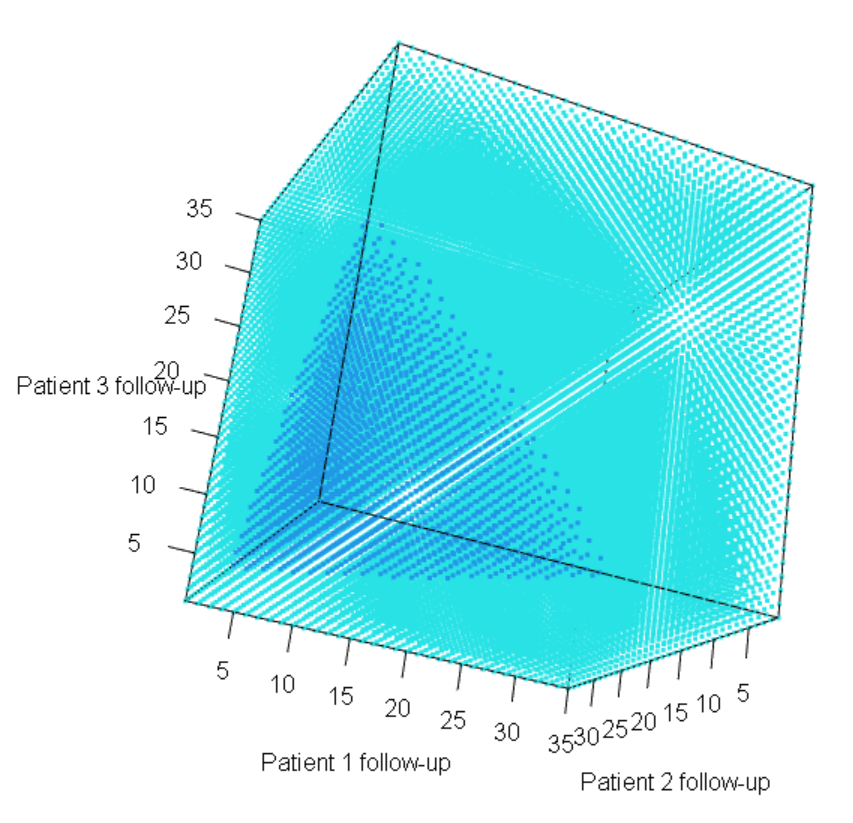
\includegraphics[width=0.85\textwidth]{TITE-DTP-c3NNN}
\end{figure}

In this example, there are 156 different pathways where the combined follow-up between the three patients is 24-26 days. By examining these pathways specifically we can define the different thresholds that are needed to make different decisions. So, if one of the three patients has a minimum of 22 days of follow-up then the model will recommend dose-level 5. This is why the minimum combined days of follow-up is 24 to recommend dose-level 5 in Table \ref{tab_tite-dtp:TITEDTP_c3NNN} as one patient will have 22 days and the other two will have one day each. In the case where one patient has a minimum follow-up of 20 or 21 days, the model will only recommend escalating to dose-level 5 if the combined follow-up of all three patients is 25. For one patient with a follow-up time between 16 and 19 days, the combined total has to be 26 to escalate to dose-level 5. There is also one pathway which includes a patient with 15 days of follow-up another with 10 days and the last patient with 1 day that escalates to dose-level 5. However every other variant of one patient having 15 days of follow-up with the combined total reaching 24-26 only escalates to dose-level 4. Out of the 156 combinations of combined follow-up between 24 and 26 days 126 recommend dose-level 4 and 30 recommend dose-level 5. 

Table \ref{tab_tite-dtp:TITEDTP_c3_Sum} combines all the different scenarios and creates a summary table of the TITE-DTPs for a cohort of three. As before we have left the overlapping combined follow-up times for the NNN scenario. Looking at the number of pathways can be quite misleading as from this table it would seem that a large number of them would end up recommending dose-level 5 however, this scenario might not be the most likely depending on what the underlying toxicity is of the dose-level. A higher number of pathways does not correlate to that outcome being more likely it just indicates that it is more complex. Therefore, extra care should be taken when interpreting TITE-DTPs. 

\begin{table}[H]
	\centering
	\caption{Summary of TITE-DTP for a cohort of three.}
	\label{tab_tite-dtp:TITEDTP_c3_Sum}
	\begin{tabular}{ccccc}
		\toprule
		\multicolumn{1}{l}{} & 				   &\multicolumn{2}{c}{Cohort 1}                       & Cohort 2 \\ 
		\cmidrule(l{3pt}r{3pt}){3-4} \cmidrule(l{3pt}r{3pt}){5-5}
		Dose                 & No. of Pathways & Outcome              & Follow-up & Dose     \\ \hline
		2                    & 1               & TTT                  &           & 1        \\ \hline
		2                    & 35              & NTT                  & 1-35      & 1        \\ \hline
		\multirow{2}{*}{2}   & 624             & \multirow{2}{*}{NNT} & 2-66      & 1        \\
		& 6               &                      & 67-70     & 2        \\ \hline
		\multirow{2}{*}{2}   & 484             & \multirow{2}{*}{NNN} & 3-26      & 4        \\
		& 7286            &                      & 24-105    & 5        \\ 
		\bottomrule
	\end{tabular}
\end{table}

Back in section \ref{tite-dtp:UsingDTPs-Calibration}, we introduced a simple trial example and produced DTPs (Table \ref{tab_tite-dtp:InitialDTPExample}). The pathways for cohort 1 in that table are the full information equivalent of the TITE-DTPs in Table \ref{tab_tite-dtp:TITEDTP_c3_Sum}. As the same trial example was used to produce both of these pathways the only difference is for one of them we have allowed the ability to use partial information in the form of the TITE-CRM and introduce a follow-up period of 35 days. In Table \ref{tab_tite-dtp:InitialDTPExample} pathways 1-16 indicate NNN which is equivalent to Table \ref{tab_tite-dtp:TITEDTP_c3_Sum} outcome of NNN when the follow-up is max for each patient i.e. 105 days of combined follow-up. In both sets of pathways we can see the recommended dose for cohort 2 is dose-level 5. The outcome where all three patients have a toxicity is exactly the same for both the DTP and TITE-DTP. For the outcome of NTT we can see the recommended dose for cohort 2 is the same in both pathways, this implies allowing for partial information doesn't change the recommendation for this cohort. When we come to compare NNT we can see that allowing for partial information does have a slightly different impact on dose recommendations. If the cohort is evaluated when there are two partial tolerances with the number of combined follow-up days being 66 or lower the model recommends dose-level 1. Contrast this to when we have full information (each patient has 35 days of follow-up with no toxicity or just the CRM version of the DTP, Table \ref{tab_tite-dtp:InitialDTPExample}) and the recommended dose is 2. TITE-DTPs also allow you to compare your design to one with full information i.e the CRM equivalent of a TITE-CRM and allow you to evaluate the length of the follow-up period and see how the dose decisions change as you move through it. 

%----------------------------------------------------------------------------------------
%	SECTION 3
%----------------------------------------------------------------------------------------

\section{Discussion}
\label{tite-dtp:Discussion}

Dose transition pathways as a tool were developed to improve communication and understanding of model-based designs. Often clinicians may not feel comfortable with having a model select doses when compared to the standard approach of a traditional and easy to follow rule-based design. DTPs try to bridge this gap and make these model-based designs more approachable. They do this by summarising model recommendations based on possible outcomes into simple pathways of dose decisions. They also can be used by the statistician to help calibrate the model and any design specifications. In particular, this helps with implementing stopping rules and investigating how escalation occurs. There is also a potential operational upside where DTPs can aid the running of a trial. By looking ahead there may be instances where regardless of any outcomes observed on the trial the dose-level won't change, in scenarios like this the need for a statistician may be lessened. 

DTPs can also be implemented as a visualisation tool to help visualise all the pathways in advance. This may have benefits in terms of raising any imminent safety concerns if certain pathways are followed. They can also be used throughout a trial's life cycle at safety committee meetings to discuss potential doses for future cohorts of patients. They are also very adaptive and are able to handle many challenging circumstances such as a change in cohort size or a patient receiving an incorrect dose. If these circumstances were to occur new DTPs could simply be calculated to account for any trial deviations. Although this is not an exclusive feature of DTPs, they are only capable of handling these scenarios because they can be accounted for in model-based designs like the CRM. 

A lot of this chapter focused on providing examples of how DTPs could be implemented specifically for a CRM design. However, the concept can easily be applied to many other model-based dose-finding trial designs such as BOIN and EffTox and even the 3+3. Implementation of these DTPs is relatively simple as well with the escalation package by Brock \cite{brockModularApproachDose2020}. It should be noted, as mentioned above, some of the flexibility of DTPs is due to the underlying designs that are used to make them. So, some challenges may be found when producing DTPs for certain types of trial designs. 

It is clear that the inclusion and use of DTPs is a net positive for dose-finding trials, not just in their design but also during the running of the trial. In the discussion section of the Yap et al. \cite{yapDoseTransitionPathways2017} paper which first introduces the idea, there is some mention of applying DTPs to TITE-CRMs. They mention the problems with patients having either partial or full tolerance and how DTPs may differ depending on how much follow-up time they achieve. One recommendation they gave was to produce the CRM equivalent DTPs, this would be useful during design stages to assess whether dose decisions change with full or partial information. 

Our work agrees with what Yap et al. \cite{yapDoseTransitionPathways2017} originally theorised. Extending DTPs to a TITE-CRM is problematic. Firstly, due to the idea of partial tolerances, trying to account for every possibility and time point a patient hasn't had a toxicity is an exponentially increasing problem. The complexity of DTPs is intrinsically linked to patients with partial tolerances as to fully build out the TITE-DTP you need to calculate every possible time point at which that patient could be observed. Then also for cohorts of more than one patient, considering the outcome where both patients experience a partial tolerance exponentially increases the number of pathways. We demonstrated that by showing the different potential DTPs for cohorts of patients from sizes one to two to three and how the number of pathways kept increasing with each iteration. 

We also found the TITE-CRM to have small inconsistencies when escalating doses. In some instances, different dose decisions were being made based on the split of follow-up time between patients for the same overall combined follow-up time. So, in our final example and TITE-DTP for a cohort of three patients we saw different recommendations when the combined amount of follow-up time between the three patients was 24, 25 or 26 days dependent on how those were split between the patients. It's not entirely obvious why this occurs, except there must exist some threshold where the TITE-CRM will escalate once one individual patient has enough follow-up and hence enough weighting. 

The examples of TITE-DTPs we provided were for only one cohort as well. Obviously, this becomes more and more difficult to deal with as we add in extra patients and cohorts. It's also not as trivial as just presenting a summary table as we did for the first cohort as well. Any additional cohort will have to take into account not only partial tolerance events from the new cohort but would have to consider every remaining possible partial tolerance event from a previous cohort. Consider one pathway from a cohort of three, N(31)N(23)N(9), all patients here experienced a partial tolerance and as their combined follow-up time adds up to 63 days we can see from the TITE-DTP in Table \ref{tab_tite-dtp:TITEDTP_c3_Sum} the dose recommendation would be dose-level 5. If we were to then recruit cohort 2 to dose-level 5 and attempt to produce more pathways we would need to check combinations for each possible amount of remaining follow-up time for the patients in the previous cohort as well as the full 35 days for each of the three new patients. So, this can essentially be thought of as a cohort of six, where some patients already have some data available. Equation \ref{eq_tite-dtp:combinations} can then be used to give us a rough estimate of how many combinations need to be considered. For a cohort of 6 patients with 35 days of follow-up, the number of combinations is $1 \times 10^{41}$. Now since we already have some data a few of these combinations are redundant but that is still an astronomical amount of pathways (for context the universe is approximately $4.3 \times 10^{17}$ seconds old). 

One way in which TITE-DTPs could work with multiple cohorts would be if previous cohorts were completed and had full information. That data could go directly into the model and you wouldn't need to consider any previous partial tolerances. When a dose decision for cohort 2 is made on partial information from cohort 1, TITE-DTPs could be created showing outcomes for cohort 3 that assume cohort 1 has full information. In practice, this may very much be the case as well depending on factors such as recruitment time and the follow-up period. 

The way DTPs are calculated the outcomes are specified and then entered into the model and then the recommended dose based on those is extracted. Those values are then used to construct the DTPs. That means for each outcome we have to specify an individual model. So, earlier in the chapter when there were 64 pathways 64 models were fitted and in the example of TITE-DTPs for a cohort of 3 we had 8436. As you increase the cohort size and the number of patients or the number of follow-up days in the trial, the number of pathways increases hence the number of models required to compute the DTP increase and the more models required the more computing time is needed. One way around this may be to stop computing once a dose-decision threshold is reached. This specifically relates to any outcomes where a partial tolerance occurs.  In the TITE-DTP example for the NNN outcome, we see anything after 27 days of combined follow-up recommends dose-level 5, We could incorporate a rule into our code that checks after each combination of follow-up days if the recommended dose changes and remains the same across every permutation of follow-up time across the patients DTPs would stop being calculated and you can assume the recommended dose will be the same. That's to say in this scenario for every combination of the three patients' follow-up time that adds up to 27 the model recommends dose-level 5 so we can assume that for any additional follow-up time the model will make the same recommendation as that is the maximum dose. This could cut down computing time on thousands of additional pathways depending on the scenario and context. 

An alternative method of producing TITE-DTPs may be to use patients' weight as a reference instead of their follow-up time. Even though weight is a function of follow-up time it might make presenting the TITE-DTPs simpler. A set of weights could be specified and pathways for those could be calculated instead. So rather than calculating pathways for N(1), N(2), ..., N(34), N you just calculate pathways when a patient is at 25\%, 50\%, 75\% and 100\% weighting. The issue with this is in order to make it interpretable you would have to back-transform the weighting. So in our example with a 35 day follow-up period and a linear weight function weightings of 25\%, 50\%, 75\% and 100\% would correspond to 8.75, 17.5, 26.25, and 35 days respectively. This might not be intuitive but it is one way to reduce the number of potential pathways. For cohorts of two or more where multiple patients are experiencing partial tolerance rather than looking at every possible combination you could just look at specific weightings. For example what is the pathway when both patients are at 50\% weight, or perhaps when one is at 75\% and the other at 25\%.  

As Yap et al. \cite{yapDoseTransitionPathways2017} suggested perhaps the easiest approach is just to assume that full tolerance will be achieved and calculate DTPs from that viewpoint. So treat the trial like a CRM and give full weighting to all the patients. This could be used as an alternative and a way to compare dose decisions made on partial information versus full information. This comparison was also made in our example and we saw how some decisions may change with only partial information. During the design stage of a trial, this may be useful in helping determine the length of any potential observation window and how dose decisions may change during it.  

In order to demonstrate TITE-DTPs we have used a relatively simple TITE-CRM trial design that doesn't include any stopping rules. Changes to any of the specifications or the inclusion of stopping rules would alter the results we produced. The observation window of 35 days that we selected was also fairly arbitrary and as discussed previously any significant increase in this value will drastically increase the number of pathways that need to be calculated. Along with that we also used a simple linear weight function. A more complex weight function would also alter the results of our pathways and depending on its complexity different features may emerge such as the inconsistencies we found. 

Overall it is possible to produce TITE-DTPs but it heavily depends on the number of days that patients can have a partial tolerance. It also depends on the size of the cohort you are evaluating. There are also some practical suggestions for how TITE-DTPs could be used during a trials design as well as it is running. Based on all these factors it appears problematic to produce TITE-DTPs for more than one cohort at a time and this will only be feasible during a trial if you can assume complete information on previous cohorts. Ultimately TITE-DTPs are still able to achieve the same aims as DTP except its ability to look ahead is a lot less. Statisticians should attempt to produce them wherever possible. However, if the scenario or trial parameters mean the TITE-DTPs is too complicated they may be more of a hindrance than a benefit.










































